\chapter[Applications]{Applications}
\label{chap:applications}

% Position the image to the right of the heading.
\vspace{-7\baselineskip} % move up
\hfill
 \begin{minipage}{0.5\textwidth}
 \centering
 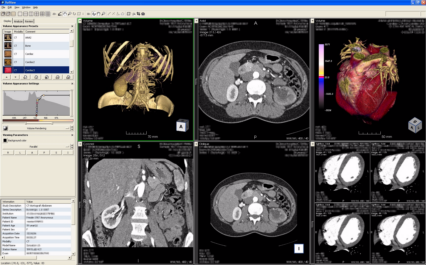
\includegraphics{VTKTextbook-275}
  \captionof*{figure}{\textit{Displaying kidney and heart CT datasets using VolView Clinical 1.0.}}
 \end{minipage}
\vspace{2\baselineskip}

\index{applications|(}
\firstletter{W}e have described the design and implementation of an extensive toolkit of visualization techniques.
In this chapter we examine several case studies to show how to use these tools to gain insight into important application areas.
These areas are medical imaging, financial visualization, modeling, computational fluid dynamics, finite element analysis, and algorithm visualization. For each case, we briefly describe the problem domain and what information we expect to obtain through visualization.
Then we craft an approach to show the results.
Many times we will extend the functionality of the Visualization Toolkit with application specific tools.
Finally, we present a sample program and show resulting images.

The visualization design process we go through is similar in each case.
First, we read or generate application--specific data and transform it into one of the data representation types in the Visualization Toolkit.
Often this first step is the most difficult one because we have to write custom computer code, and decide what form of visualization data to use.
In the next step, we choose visualizations for the relevant data within the application.
Sometimes this means choosing or creating models corresponding to the physical structure. Examples include spheres for atoms, polygonal surfaces to model physical objects, or computational surfaces to model flow boundaries.
Other times we generate more abstract models, such as isosurfaces or glyphs, corresponding to important application data.
In the last step we combine the physical components with the abstract components to create a visualization that aids the user in understanding the data.

\section{3D Medical Imaging}
\index{applications!medical imaging|(}\index{medical imaging!application|(}

Radiology is a medical discipline that deals with images of human anatomy.
These images come from a variety of medical imaging devices, including X--ray, X--ray Computed Tomography\index{Computed Tomography}\index{CT|see {Computed Tomography}}), Magnetic Resonance Imaging (MRI)\index{MRI}, and ultrasound. Each imaging technique, called an imaging modality, has particular diagnostic strengths.

\begin{figure}[!htb]
	\centering
	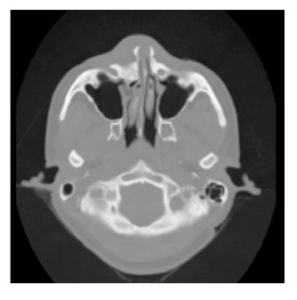
\includegraphics[width=0.8\textwidth]{Figure12-1}
	\caption{A CT slice through a human head.}
	\label{fig:Figure12-1}
\end{figure}

This case study deals with CT data. Computed tomography measures the attenuation of X--rays as they pass through the body. A CT image consists of levels of gray that vary from black (for air), to gray (for soft tissue), to white (for bone).  Figure \ref{fig:Figure12-1} shows a CT cross section through a head. This slice is taken perpendicular to the spine approximately through the middle of the ears.  The gray boundary around the head clearly shows the ears and bridge of the nose. The dark regions on the interior of the slice are the nasal passages and ear canals. The bright areas are bone. This study contains 93 such slices, spaced $1.5$ mm apart. Each slice has $256^2$ pixels spaced 0.8 mm apart with $12$ bits of gray level.

Our challenge is to take this gray scale data (over $12$ megabytes) and convert it into information that will aid the surgeon. Fortunately, our visualization toolkit has just the right techniques. We will use isocontouring techniques to extract the skin and bone surfaces and display orthogonal cross--sections to put the isosurface in context. From experience we know that a density value of $500$ will define the air/skin boundary, and a value of 1150 will define the soft tissue/bone boundary. In VTK terminology, medical imaging slice data is image data. Recall from Chapter 5: \nameref{chap:basic_data_representation} that for image data, the topology and geometry of the data is implicitly known, requiring only dimensions, an origin, and the data spacing.

The steps we follow in this case study are common to many three--dimensional medical studies.
\begin{enumerate}

    \item Read the input.

    \item For each anatomical feature of interest, create an isosurface.

    \item Transform the models from patient space to world space.

    \item Render the models.

\end{enumerate}

This case study describes in detail how to read input data and extract anatomical features using iso--contouring. Orthogonal planes will be shown using a texture-based technique. Along the way we will also show you how to render the data. We finish with a brief discussion of medical data transformations. This complete source code for the examples shown in this section are available from 
\href{https://lorensen.github.io/VTKExamples/site/Cxx/Medical/MedicalDemo1/}{MedicalDemo1.cxx} or \href{https://lorensen.github.io/VTKExamples/site/Python/Medical/MedicalDemo1/}{MedicalDemo1.py}, 
\href{https://lorensen.github.io/VTKExamples/site/Cxx/Medical/MedicalDemo2/}{MedicalDemo2.cxx} or \href{https://lorensen.github.io/VTKExamples/site/Python/Medical/MedicalDemo2/}{MedicalDemo2.py}, and
\href{https://lorensen.github.io/VTKExamples/site/Cxx/Medical/MedicalDemo3/}{MedicalDemo3.cxx} or \href{https://lorensen.github.io/VTKExamples/site/Python/Medical/MedicalDemo3/}{MedicalDemo3.py}.

\subsection{Read the Input}

Medical images come in many flavors of file formats. This study is stored as flat files without header information. Each 16--bit pixel is stored with little-endian byte order. Also, as is often the case, each slice is stored in a separate file with the file suffix being the slice number of the form \texttt{prefix.1}, \texttt{prefix.2}, and so on. Medical imaging files often have a header of a certain size before the image data starts. The size of the header varies from file format to file format. Finally, another complication is that sometimes one or more bits in each 16-bit pixel is used to mark connectivity between voxels. It is important to be able to mask out bits as they are read.

VTK provides several image readers including one that can read raw formats of the type described above --- vtkVolume16Reader. To read this data we instantiate the class and set the appropriate instance variables as follows.

\begin{lstlisting}[language=C++, caption={Reading raw formatted files.}]
vtkVolume16Reader *v16 = vtkVolume16Reader::New();
  v16->SetDataDimensions (64,64); v16->SetImageRange (1,93);
  v16->SetDataByteOrderToLittleEndian();
  v16->SetFilePrefix ("headsq/quarter");
  v16->SetDataSpacing (3.2, 3.2, 1.5);
\end{lstlisting}

The FilePrefix and FilePattern instance variable work together to produce the name of files in a series of slices. The FilePattern --- which by default is \%s.\%d --- generates the filename to read by performing a C-language sprintf() of the FilePrefix and the current file number into the FilePattern format specifier.

\subsection{Create an Isosurface}

We can choose from three techniques for isosurface visualization: volume rendering\index{volume rendering}, marching cubes\index{marching cubes!aplication}, and dividing cubes\index{dividing cubes}. We assume that we want to interact with our data at the highest possible speed, so we will not use volume rendering. We prefer marching cubes if we have polygonal rendering hardware available, or if we need to move up close to or inside the extracted surfaces. Even with hardware assisted rendering, we may have to reduce the polygon count to get reasonable rendering speeds. Dividing cubes is appropriate for software rendering. For this application we'll use marching cubes.

For medical volumes, marching cubes generates a large number of triangles. To be practical,  we'll do this case study with a reduced resolution dataset. We took the original $256^2$ data and reduced it to $64^2$ slices by averaging neighboring pixels twice in the slice plane. We call the resulting dataset \emph{quarter} since it has 1/4 the resolution of the original data. We adjust the DataSpacing for the reduced resolution dataset to 3.2 mm per pixel. Our first program will generate an isosurface\index{isosurface!application} for the skin.

The flow in the program is similar to most VTK applications.

\begin{itemize}

	\item Generate some data.

	\item Process it with filters.

	\item Create a mapper to generate rendering primitives.

	\item Create actors for all mappers.

	\item Create actors for all mappers.

\end{itemize}

The filter we have chosen to use is vtkMarchingCubes\index{vtkMarchingCubes!application}. We could also use vtkContourFilter since it will automatically create an instance of vtkMarchingCubes as it delegates to the fastest subclass for a particular dataset type. The class vtkPolyDataNormals is used to generate nice surface normals for the data. vtkMarchingCubes can also generate normals, but sometimes better results are achieved when the normals are directly from the surface (vtkPolyDataNormals ) versus from the data (vtkMarchingCubes ). To complete this example, we take the output from the isosurface generator vtkMarchingCubes and connect it to a mapper and actor via
vtkPolyDataMapper and vtkActor\index{vtkActor!application}. The C++ code follows.

\begin{lstlisting}[language=C++, caption={Creating an isosurface.}, escapechar=\$]
vtkContourFilter *skinExtractor = vtkContourFilter::New();
  skinExtractor->SetInputConnection(v16->GetOutputPort());
  skinExtractor->SetValue(0, 500);

vtkPolyDataNormals *skinNormals = vtkPolyDataNormals::New();
  skinNormals->SetInputConnection(skinExtractor->GetOutputPort());
  skinNormals->SetFeatureAngle(60.0);

vtkPolyDataMapper *skinMapper = vtkPolyDataMapper::New();
  skinMapper->SetInputConnection(skinNormals->GetOutputPort());
  skinMapper->ScalarVisibilityOff();

vtkActor *skin = vtkActor::New();
  skin->SetMapper(skinMapper);

vtkOutlineFilter *outlineData = vtkOutlineFilter::New();
  outlineData->SetInputConnection(v16->GetOutputPort());
  vtkPolyDataMapper *mapOutline = vtkPolyDataMapper::New();
  mapOutline->SetInputConnection(outlineData->GetOutputPort());

vtkActor *outline = vtkActor::New();
  outline->SetMapper(mapOutline);
  outline->GetProperty()->SetColor(0,0,0);

vtkCamera *aCamera = vtkCamera::New();
  aCamera->SetViewUp (0, 0, -1);
  aCamera->SetPosition (0, 1, 0);
  aCamera->SetFocalPoint (0, 0, 0);
  aCamera->ComputeViewPlaneNormal();

  aRenderer->AddActor(outline);
  aRenderer->AddActor(skin);
  aRenderer->SetActiveCamera(aCamera);
  aRenderer->ResetCamera ();

  aCamera->Dolly(1.5);

  aRenderer->SetBackground(1,1,1);

  renWin->SetSize(640, 480);

  aRenderer->ResetCameraClippingRange ();

  // Initialize the event loop and then start it.
  iren->Initialize();
  iren->Start();
\end{lstlisting}

\begin{figure}[!htb]
	\centering
	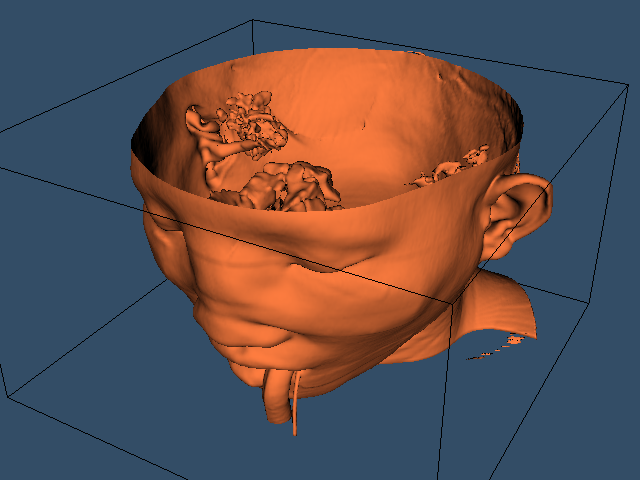
\includegraphics[width=0.8\textwidth]{Figure12-2}
	\caption{The skin extracted from a CT dataset of the head.(\href{https://lorensen.github.io/VTKExamples/site/Cxx/Medical/MedicalDemo1/}{MedicalDemo1.cxx}) and (\href{https://lorensen.github.io/VTKExamples/site/Python/Medical/MedicalDemo1/}{MedicalDemo1.py})}
	\label{fig:Figure12-2}
\end{figure}

To provide context for the isosurface an outline is created around the data. An initial view is set up  in a window size of $640 \times 480$ pixels. Since the dolly command moves the camera towards the data, the clipping planes are reset to insure that the isosurface is
completely visible. Figure \ref{fig:Figure12-2} shows the resulting image of the patient's skin.

We can improve this visualization in a number of ways. First, we can choose a more appropriate color (and other surface properties) for the skin. We use the vtkProperty method SetDiffuseColor() to set the skin color to a fleshy tone. We also add a specular component to the skin surface. Next, we can add additional isosurfaces corresponding to various anatomical features. Here we choose to extract the bone surface by adding an additional pipeline segment. This consists of the filters vtkMarchingCubes, vtkPolyDataMapper, and vtkActor, just as we did with the skin. Finally, to improve rendering performance on our system, we create triangle strips from the output of the contouring process. This requires adding vtkStripper.

\begin{figure}[!htb]
	\centering
	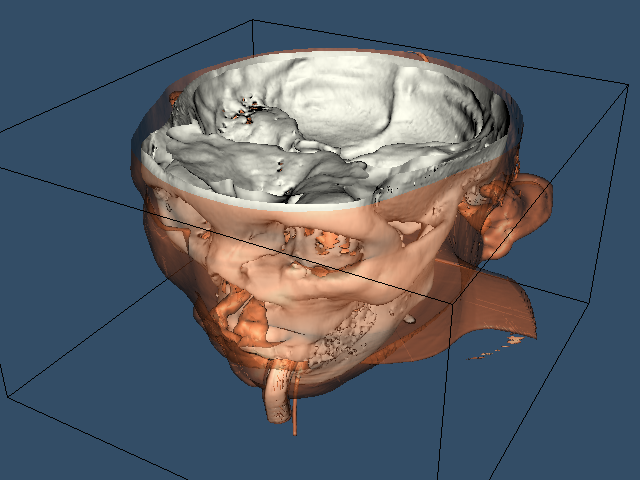
\includegraphics[width=0.8\textwidth]{Figure12-3}
	\caption{Skin and bone isosurfaces.(\href{https://lorensen.github.io/VTKExamples/site/Cxx/Medical/MedicalDemo2/}{MedicalDemo2.cxx}) and (\href{https://lorensen.github.io/VTKExamples/site/Python/Medical/MedicalDemo2/}{MedicalDemo2.py})}
	\label{fig:Figure12-3}
\end{figure}

Figure \ref{fig:Figure12-3} shows the resulting image, and the following is the C++ code for the pipeline.

\begin{lstlisting}[language=C++, caption={Improving the visualizarion of the isosurface.}]
vtkActor *skin = vtkActor::New();
  skin->SetMapper(skinMapper);
  skin->GetProperty()->SetDiffuseColor(1, .49, .25);
  skin->GetProperty()->SetSpecular(.3);
  skin->GetProperty()->SetSpecularPower(20);
  skin->GetProperty()->SetOpacity(1.0);

vtkContourFilter *boneExtractor = vtkContourFilter::New();
  boneExtractor->SetInputConnection(v16->GetOutputPort());
  boneExtractor->SetValue(0, 1150);

vtkPolyDataNormals *boneNormals = vtkPolyDataNormals::New();
  boneNormals->SetInputConnection(boneExtractor->GetOutputPort());
  boneNormals->SetFeatureAngle(60.0);

vtkStripper *boneStripper = vtkStripper::New();
  boneStripper->SetInputConnection(boneNormals->GetOutputPort());

vtkPolyDataMapper *boneMapper = vtkPolyDataMapper::New();
  boneMapper->SetInputConnection(boneStripper->GetOutputPort());
  boneMapper->ScalarVisibilityOff();

vtkActor *bone = vtkActor::New(); bone->SetMapper(boneMapper);
  bone->GetProperty()->SetDiffuseColor(1, 1, .9412);
\end{lstlisting}

The \emph{Visualization Toolkit} provides other useful techniques besides isocontouring for exploring volume data. One popular technique used in medical imaging is to view orthogonal slices, or planes, through the data. Because computer graphics hardware supports texture mapping, an approach using texture mapping gives the best result in terms or interactive performance.

We will extract three orthogonal planes corresponding to the axial, sagittal, and coronal cross sections that are familiar to radiologists. The axial plane is perpendicular to the patient's neck, sagittal passes from left to right, and coronal passes from front to back. For illustrative purposes, we render each of these planes with a different color lookup table. For the sagittal plane, we use a gray scale. The coronal and axial planes vary the saturation and hue table, respectively. We combine this with a translucent rendering of the skin (we turn off the bone with the C++ statement bone->VisibilityOff() ). The following VTK code creates the three lookup tables that are used in the texture mapping process.

\begin{lstlisting}[language=C++, caption={Lookup tables for the sectioning planes.}, escapechar=\$]
vtkLookupTable$\index{vtkLookupTable!application}$ *bwLut = vtkLookupTable::New();
  bwLut->SetTableRange (0, 2000);
  bwLut->SetSaturationRange (0, 0);
  bwLut->SetHueRange (0, 0);
  bwLut->SetValueRange (0, 1);

vtkLookupTable *hueLut = vtkLookupTable::New();
  hueLut->SetTableRange (0, 2000);
  hueLut->SetHueRange (0, 1);
  hueLut->SetSaturationRange (1, 1);
  hueLut->SetValueRange (1, 1);

vtkLookupTable *satLut = vtkLookupTable::New();
  satLut->SetTableRange (0, 2000);
  satLut->SetHueRange (.6, .6);
  satLut->SetSaturationRange (0, 1);
  satLut->SetValueRange (1, 1);
\end{lstlisting}

\begin{figure}[!htb]
	\centering
	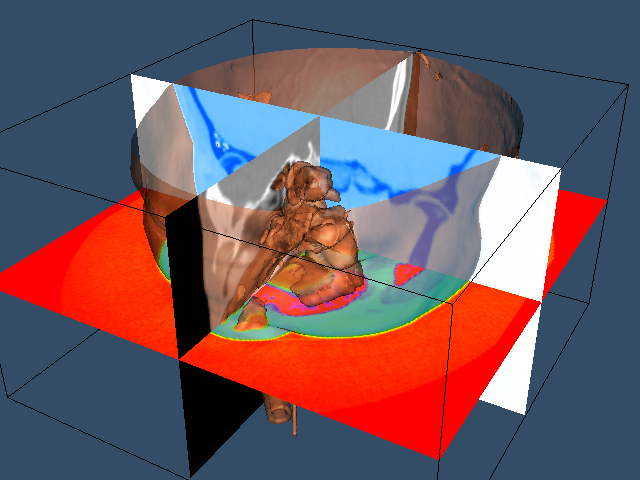
\includegraphics[width=0.8\textwidth]{Figure12-4}
	\caption{Composite image of three planes and translucent skin.(\href{https://lorensen.github.io/VTKExamples/site/Cxx/Medical/MedicalDemo3/}{MedicalDemo3.cxx}) and (\href{https://lorensen.github.io/VTKExamples/site/Python/Medical/MedicalDemo3/}{MedicalDemo3.py})}
	\label{fig:Figure12-4}
\end{figure}

The image data is mapped to colors using the filter vtkImageMapToColors\index{vtkImageMapToColors} in combination with the lookup tables created above. The actual display of the slice is performed with vtkImageActor\index{vtkImageActor} (see ``Assemblies and Other Types of vtkProp'' on page \pageref{subsubsec:assemblies_vtkprop} for more information). This class conveniently combines a quadrilateral, polygon plane with a texture map. vtkImageActor requires image data of type unsigned char, which the class vtkImageMapToColors conveniently provides. To avoid copying the data and to specify the 2D texture to use, the DisplayExtent of each vtkImageActor is set appropriately. The C++ code is as follows:

\begin{lstlisting}[language=C++, caption={Mapping the image data and displaying the image slices.}, escapechar=\$]
// saggital

vtkImageMapToColors$\index{vtkImageMapToColors!application}$ *saggitalColors = vtkImageMapToColors::New();
  saggitalColors->SetInputConnection(v16->GetOutputPort());
  saggitalColors->SetLookupTable(bwLut);

vtkImageActor$\index{vtkImageActor!application}$ *saggital = vtkImageActor::New();
  saggital->SetInputConnection(saggitalColors->GetOutputPort());
  saggital->SetDisplayExtent(32,32, 0,63, 0,92);

// axial

vtkImageMapToColors *axialColors = vtkImageMapToColors::New();
  axialColors->SetInputConnection(v16->GetOutputPort());
  axialColors->SetLookupTable(hueLut);

vtkImageActor *axial = vtkImageActor::New();
  axial->SetInputConnection(axialColors->GetOutputPort());
  axial->SetDisplayExtent(0,63, 0,63, 46,46);

// coronal

vtkImageMapToColors *coronalColors = vtkImageMapToColors::New();
  coronalColors->SetInputConnection(v16->GetOutputPort());
  coronalColors->SetLookupTable(satLut);

vtkImageActor *coronal = vtkImageActor::New();
  coronal->SetInputConnection(coronalColors->GetOutputPort());
  coronal->SetDisplayExtent(0,63, 32,32, 0,92);

  aRenderer->AddActor(outline);
  aRenderer->AddActor(saggital);
  aRenderer->AddActor(axial);
  aRenderer->AddActor(coronal);
  aRenderer->AddActor(bone);
  aRenderer->AddActor(skin);
\end{lstlisting}

Figure \ref{fig:Figure12-4} shows the resulting composite image.

In this example, the actor named skin is rendered last because we are using a translucent surface. Recall from ``Transparency and Alpha Values'' on page \pageref{sec:transparency_alpha} that we must order the polygons  composing transparent surfaces for proper results. We render the skin last by adding it to aRenderer's actor list last.

We need to make one last point about processing medical imaging data. Medical images can be acquired in a variety of orders that refer to the relationship of consecutive slices to the patient. Radiologists view an image as though they were looking at the patient's feet. This means that on the display, the patient's left appears on the right. For CT there are two standard orders: top to bottom or bottom to top. In a top to bottom acquisition, slice \emph{i} is farther from the patient's feet than slice emph{i} - 1. Why do we worry about this order? It is imperative in medical applications that we retain the left / right relationship. Ignoring the slice acquisition order can result in a flipping of left and right. To correct this, we need to transform either the original dataset or the geometry we have extracted. (See ``Exercises'' on page \pageref{exercises:ch_12} for more information.) Also, you may wish to examine the implementation of the classes vtkVolume16Reader and vtkVolumeReader (the superclass of vtkVolume16Reader). These classes have special methods that deal with transforming image data.
\index{applications!medical imaging|)}\index{medical imaging!application|)}

\section{Creating Models from Segmented Volume Data}
\index{applications!segmented volume data|(}\index{segmented volume data!application|(}\index{Tcl!application|(}

The previous example described how to create models from gray--scale medical imaging data. The techniques for extracting bone and skin models is straightforward compared to the task of generating models of other soft tissue. The reason is that magnetic resonance and, to some extent, computed tomography, generates similar gray-scale values for different tissue types. For example, the liver and kidney in a medical computed tomography volume often have overlapping intensities. Likewise, many different tissues in the brain have overlapping intensities when viewed with magnetic resonance imaging. To deal with these problems researchers apply a process called \emph{segmentation}\index{segmentation} to identify different tissues. These processes vary in sophistication from almost completely automatic methods to manual tracing of images. Segmentation continues to be a hot research area. Although the segmentation process itself is beyond the scope of this text, in this case study we show how to process segmented medical data.

For our purposes we assume that someone (or many graduate students) have laboriously labeled each pixel in each slice of a volume of data with a tissue identifier. This identifier is an integer number that describes which tissue class each pixel belongs to. For example, we may be given a series of MRI slices of the knee with tissue numbers defining the meniscus, femur, muscles, and so forth. Figure \ref{fig:Figure12-5} shows two representations of a slice from a volume acquired from a patient's knee. The image on the left is the original MRI slice; the image on the right contains tissue labels for a number of important organs. The bottom image is a composite of the two images.

\begin{figure}[!htb]
	\floatbox[{\capbeside\thisfloatsetup{capbesideposition={left,center},capbesidewidth=0.3\textwidth}}]{figure}[\FBwidth]
	{\caption{Magnetic Resonance Image of a knee(left); segmented tissue(right); composite (bottom).(Data and segmentation courtesy of Brigham and Women's Hospital Surgical Planning Lab.}\label{fig:Figure12-5}}
	{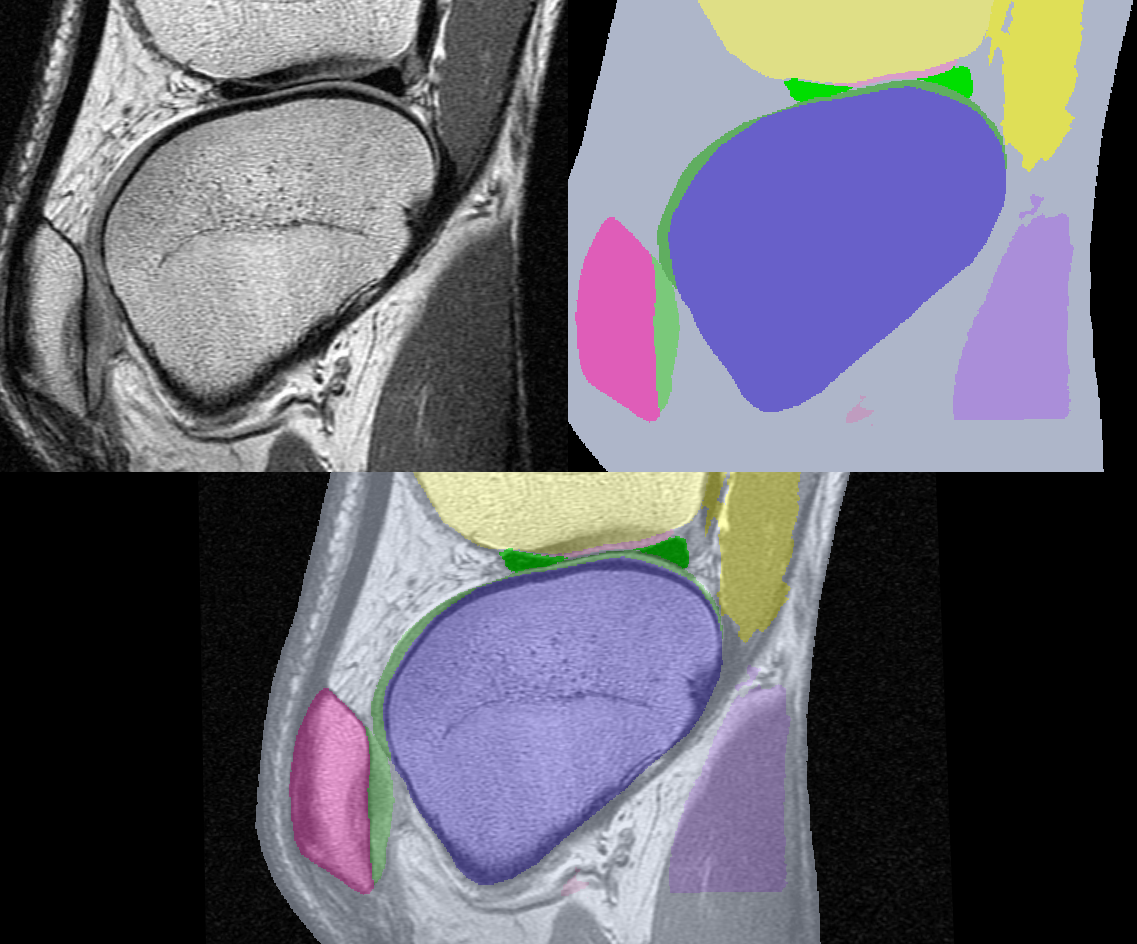
\includegraphics[width=0.7\textwidth]{Figure12-5}}
\end{figure}

Notice the difference in the information presented by each representation. The original slice shows gradual changes at organ borders, while the segmented slice has abrupt changes. The images we processed in the previous CT example used marching cubes isocontouring algorithm and an intensity threshold to extract the isosurfaces\index{isosurface!application}. The segmented study we present has integer labels that have a somewhat arbitrary numeric value. Our goal in this example is to somehow take the tissue labels and create grayscale slices that we can process with the same techniques we used previously. Another goal is to show how image processing and visualization can work together in an application.

\subsection{The Virtual Frog}

\begin{figure}[!htb]
	\floatbox[{\capbeside\thisfloatsetup{capbesideposition={right,center},capbesidewidth=0.3\textwidth}}]{figure}[\FBwidth]
	{\caption{Photographic slice of frog (upper left), segmented frog (upper right) and composite of photo and segmentation (bottom). The purple color represents the stomach and the kidneys are yellow.(\href{https://lorensen.github.io/VTKExamples/site/Cxx/Visualization/TestFrogSlice/}{TestFrogSlice.cxx}) and (\href{https://lorensen.github.io/VTKExamples/site/Python/Visualization/TestFrogSlice/}{TestFrogSlice.py})}\label{fig:Figure12-6}}
	{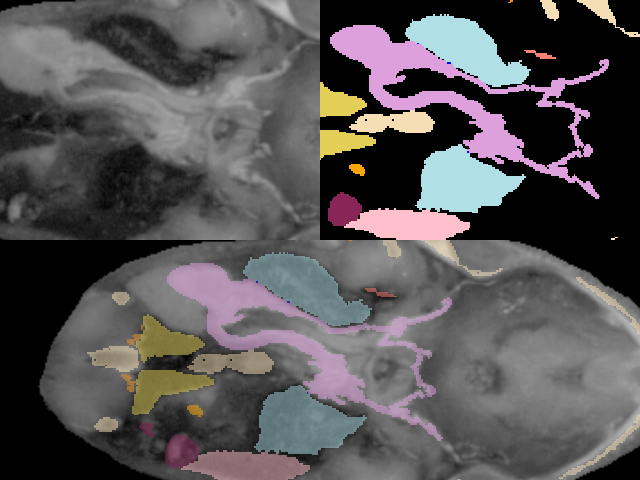
\includegraphics[width=0.7\textwidth]{Figure12-6}}
\end{figure}

To demonstrate the processing of segmented data we will use a dataset derived from a frog. This data was prepared at Lawrence Berkeley National Laboratories and is included with their permission on the CD--ROM accompanying this book. The data was acquired by physically slicing the frog and photographing the slices. The original segmented data is in the form of tissue masks with one file per tissue. There are $136$ slices per tissue and $15$ different tissues. Each slice is $470 \times 500$ pixels. (To accommodate the volume readers we have in VTK, we processed the mask files and combined them all in one file for each slice.) We used integer numbers $1$ -- $15$ to represent the 15 tissues. Figure \ref{fig:Figure12-6} shows an original slice, a labeled slice, and a composite of the two representations.

Before we describe the process to go from binary labeled tissues to gray--scale data suitable for isosurface extraction, compare the two images of the frog's brain shown in Figure \ref{fig:Figure12-7}. On the left is a surface extracted using a binary labeling of the brain. The right image was created using the visualization pipeline that we will develop in this example.

\begin{figure}[!htb]
	\centering
	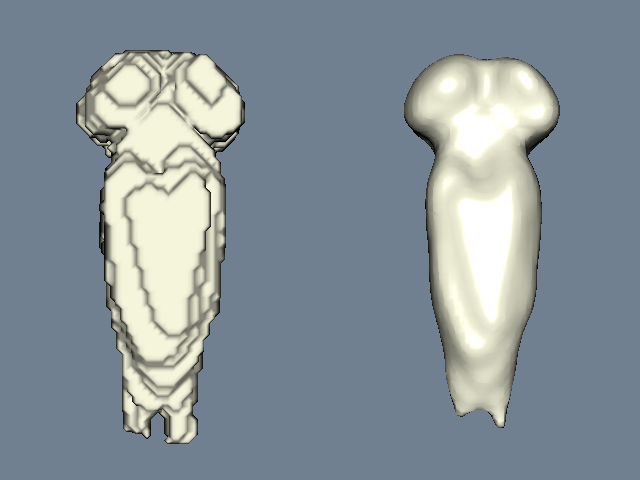
\includegraphics[width=0.8\textwidth]{Figure12-7}
	\caption{The frog's brain. Model extracted without smoothing (left) and with smoothing (right).(\href{https://lorensen.github.io/VTKExamples/site/Cxx/Visualization/ViewFrogBoth/}{ViewFrogBoth.cxx}) and (\href{https://lorensen.github.io/VTKExamples/site/Python/Visualization/ViewFrogBoth/}{ViewFrogBoth.py})}
	\label{fig:Figure12-7}
\end{figure}

\subsection{Developing a Strategy}

In the last example, we used C++ and created a program that was tailored to extract two surfaces: one of the skin and one of the bone. All the parameters for the surface extraction were hardcoded in the source. Since our frog has 15 different tissues; we seek a more general solution to this problem. We may have to experiment with a number of different parameters for a number of visualization and imaging filters. Our goal is to develop a general pipeline that will work not only our 15 tissues but on other medical datasets as well. We'll design the program to work with a set of user--specified parameters to control the elements of the pipeline. A reasonable description might look like:

\begin{lstlisting}[language=TCL, caption={User specified parameters to control the elements of the pipeline.}]
SLICE_ORDER hfsi
ROWS 470
COLUMNS 500
STUDY ../frogMasks/frogTissue
PIXEL_SIZE 1
SPACING 1.5
\end{lstlisting}

plus possibly many more parameters to control decimation, smoothing, and so forth. Working in C++, we would have to design the format of the file and write code to interpret the statements. We make the job easier here by using Tcl interpreter. Another decision is to separate the modelling from the rendering. Our script will generate models in a ``batch'' mode. We will run one VTK Tcl script for each tissue. That script will create a \texttt{.vtk} output file containing the polygonal representation of each tissue. Later, we can render the models with a separate script.

\subsection{Overview of the Pipeline}

Figure \ref{fig:Figure12-8} shows the design of the pipeline. This generic pipeline has been developed over the years in our laboratory and in the Brigham and Women's Hospital Surgical Planning Lab. We find that it produces reasonable models from segmented datasets. Do not be intimidated by the number of filters (twelve in all). Before we developed VTK, we did similar processing with a hodgepodge of programs all written with different interfaces. We used intermediate files to pass data from one filter to the next. The new pipeline, implemented in VTK, is more efficient in time and computing resources.

\begin{figure}[htb]
	\begin{subfigure}[h]{0.36\linewidth}
		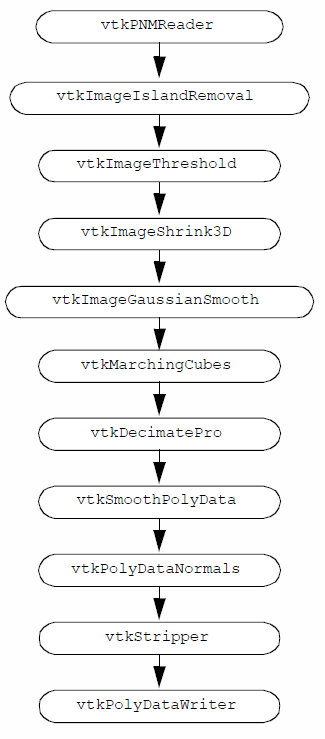
\includegraphics[width=0.96\linewidth]{Figure12-8a}
		\caption*{}
		\label{fig:Figure12-8a}
	\end{subfigure}
	\hfill
	\begin{subfigure}[h]{0.36\linewidth}
		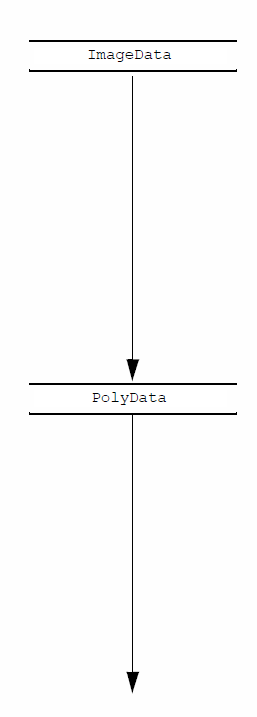
\includegraphics[width=0.96\linewidth]{Figure12-8b}
		\caption*{}
		\label{fig:Figure12-8b}
	\end{subfigure}
	\caption{The segmented volume to triangle pipeline. Volume passes through image pipeline before isosurface extraction.}\label{fig:Figure12-8}
\end{figure}

\subsection{Read the Segmented Volume Data}

We assume here that all the data to be processed was acquired with a constant center landmark. In VTK, the origin of the data applies to the lower left of an image volume. In this pipeline, we calculate the origin such that the \emph{x,y} center of the volume will be $(0,0)$. The DataSpacing describes the size of each pixel and the distance between slices. DataVOI selects a volume of interest (VOI). A VOI lets us select areas of interest, sometimes eliminating extraneous structures like the CT table bed. For the frog, we have written a small C program that reads the tissue label file and finds the volume of interest for each tissue.

The SetTransform() method defines how to arrange the data in memory. Medical images can be acquired in a variety of orders. For example, in CT, the data can be gathered from top to bottom (superior to inferior), or bottom to top (inferior to superior). In addition, MRI data can be acquired from left to right, right to left, front-to-back (anterior to posterior) or back-to-front. This filter transforms triangle vertices such that the resulting models will all ``face'' the viewer with a view up of $(0,-1,0)$, looking down the positive \emph{z} axis. Also, proper left-right correspondence will be maintained. That means the patient's left will always be left on the generated models. Look in \texttt{SliceOrder.tcl} to see the permutations and rotations for each order.

All the other parameters are self-explanatory except for the last. In this script, we know that the pipeline will only be executed once. To conserve memory, we invoke the ReleaseDataFlagOn() method. This allows the VTK pipeline to release data once it has been processed by a filter. For large medical datasets, this can mean the difference between being able to process a dataset or not.

\begin{lstlisting}[language=TCL, caption={Read the Segmented Volume Data.}]
set originx [expr ( $COLUMNS / 2.0 ) * $PIXEL_SIZE * -1.0]
set originy [expr ( $ROWS / 2.0 ) * $PIXEL_SIZE * -1.0]
vtkPNMReader reader
  reader SetFilePrefix $STUDY
  reader SetDataSpacing $PIXEL_SIZE $PIXEL_SIZE $SPACING
  reader SetDataOrigin $originx $originy
[expr $START_SLICE * $SPACING]
  reader SetDataVOI $VOI
  reader SetTransform $SLICE_ORDER
  [reader GetOutput] ReleaseDataFlagOn
\end{lstlisting}

\subsection{Remove Islands}

Some segmentation techniques, especially those that are automatic, may generate islands of misclassified voxels. This filter looks for connected pixels with the ISLAND\_REPLACE label, and if the number of connected pixels is less than ISLAND\_AREA, it replaces them with the label TISSUE. Note that this filter is only executed if ISLAND\_REPLACE is positive.

\begin{lstlisting}[language=TCL, caption={Remove Islands.}, escapechar=\%]
set lastConnection reader
if {$ISLAND_REPLACE = 0} {
  vtkImageIslandRemoval2D%\index{vtkImageIslandRemoval2D!application}% islandRemover
    islandRemover SetAreaThreshold $ISLAND_AREA
    islandRemover SetIslandValue $ISLAND_REPLACE
    islandRemover SetReplaceValue $TISSUE
    islandRemover SetInputConnection [$lastConnection GetOutputPort]
  set lastConnection islandRemover
}
\end{lstlisting}

\subsection{Select a Tissue}

The rest of the pipeline requires gray--scale data. To convert the volume that now contains integer tissue labels to a gray--scale volume containing only one tissue, we use the threshold filter to set all pixels with the value TISSUE (the tissue of choice for this pipeline) to $255$ and all other pixels to $0$. The choice of $255$ is somewhat arbitrary.

\begin{lstlisting}[language=TCL, caption={Select a Tissue.}, escapechar=\%]
vtkImageThreshold%\index{vtkImageThreshold!application}% selectTissue
  selectTissue ThresholdBetween $TISSUE $TISSUE
  selectTissue SetInValue 255
  selectTissue SetOutValue 0
  selectTissue SetInputConnection [$lastConnection GetOutputPort]
\end{lstlisting}

\subsection{Resample the Volume}

Lower resolution volumes produce fewer polygons. For experimentation we often reduce the resolution of the data with this filter. However, details can be lost during this process. Averaging creates new pixels in the resampled volume by averaging neighboring pixels. If averaging is turned off, every SAMPLE\_RATE pixel will be passed through to the output.

\begin{lstlisting}[language=TCL, caption={Resample the Volume.}, escapechar=\%]
vtkImageShrink3D%\index{vtkImageShrink3D!application}% shrinker
  shrinker SetInputConnection [selectTissue GetOutputPort] eval
  shrinker SetShrinkFactors $SAMPLE_RATE
  shrinker AveragingOn
\end{lstlisting}

\subsection{Smooth the Volume Data}

To this point, unless we have resampled the data, the volume is labeled with a value of $255$ in pixels of the selected tissue and $0$ elsewhere. This ``binary'' volume would produce stepped surfaces if we did not blur it. The Gaussian kernel specified in this filter accomplishes the smoothing we require to extract surfaces. The amount of smoothing is controlled by  GAUSSIAN\_STANDARD\_DEVIATION that can be independently specified for each axis of the volume data. We only run this filter if some smoothing is requested,

\begin{lstlisting}[language=TCL, caption={Smooth the Volume Data.}, escapechar=\%]
set lastConnection shrinker
if {$GAUSSIAN_STANDARD_DEVIATION != "0 0 0"} {
  vtkImageGaussianSmooth%\index{vtkImageGaussianSmooth!application}% gaussian
  gaussian SetDimensionality 3
  gaussian SetStandardDeviation $GAUSSIAN_STANDARD_DEVIATION gaussian
  SetRadiusFactor 1
  gaussian SetInputConnection [shrinker GetOutputPort]
  set lastConnection gaussian
}
\end{lstlisting}

\subsection{Generate Triangles}

Now we can process the volume with marching cubes\index{marching cubes!aplication} just as though we had obtained gray--scale data from a scanner. We added a few more bells and whistles to the pipeline. The filter runs faster if we turn off gradient and normal calculations. Marching cubes normally calculates vertex normals from the gradient of the volume data. In our pipeline, we have concocted a gray--scale representation and will subsequently decimate the triangle mesh and smooth the resulting vertices. This processing invalidates the normals that are calculated by marching cubes. 

\begin{lstlisting}[language=TCL, caption={Generate Triangles.}, escapechar=\%]
vtkMarchingCubes%\index{vtkMarchingCubes!application}% mcubes
  mcubes SetInputConnection [toStructuredPoints GetOutputPort]
  mcubes ComputeScalarsOff
  mcubes ComputeGradientsOff
  mcubes ComputeNormalsOff
  eval mcubes SetValue 0 $VALUE
  [mcubes GetOutput] ReleaseDataFlagOn
\end{lstlisting}

\subsection{Reduce the Number of Triangles}
There are often many more triangles generated by the isosurfacing algorithm than we need for rendering. Here we reduce the triangle count by eliminating triangle vertices that lie within a user--specified distance to the plane formed by neighboring vertices. We preserve any edges of triangles that are considered ``features''.

\begin{lstlisting}[language=TCL, caption={Reduce the Number of Triangles.}, escapechar=\%]
vtkDecimatePro%\index{vtkDecimatePro!application}% decimator
  decimator SetInputConnection [mcubes GetOutputPort]
  eval decimator SetFeatureAngle $DECIMATE_ANGLE
  decimator PreserveTopologyOn
  decimator SetTargetReduction $DECIMATE_REDUCTION
  [decimator GetOutput] ReleaseDataFlagOn
\end{lstlisting}

\subsection{Smooth the Triangle Vertices}

This filter uses Laplacian smoothing described in ``Mesh Smoothing'' on page \pageref{subsec:mesh_smoothing} to adjust triangle vertices as an ``average'' of neighboring vertices. Typically, the movement will be less than a voxel.

Of course we have already smoothed the image data with a Gaussian kernel so this step may not give much improvement; however, models that are heavily decimated can sometimes be improved with additional polygonal smoothing.

\begin{lstlisting}[language=TCL, caption={Smooth the Triangle Vertices.}]
vtkSmoothPolyDataFilter smoother
  smoother SetInputConnection [decimator GetOutputPort]
  eval smoother SetNumberOfIterations $SMOOTH_ITERATIONS
  eval smoother SetRelaxationFactor $SMOOTH_FACTOR
  eval smoother SetFeatureAngle $SMOOTH_ANGLE
  smoother FeatureEdgeSmoothingOff
  smoother BoundarySmoothingOff
  smoother SetConvergence 0
  [smoother GetOutput] ReleaseDataFlagOn
\end{lstlisting}

\subsection{Generate Normals}
To generate smooth shaded models during rendering, we need normals at each vertex. As in decimation, sharp edges can be retained by setting the feature angle.

\begin{lstlisting}[language=TCL, caption={Generate Normals.}]
vtkPolyDataNormals normals
  normals SetInputConnection
  [smoother GetOutputPort] eval normals
  SetFeatureAngle $FEATURE_ANGLE
  [normals GetOutput] ReleaseDataFlagOn
\end{lstlisting}

\subsection{Generate Triangle Strips}

Triangle strips are a compact representation of large numbers of triangles. This filter processes our independent triangles before we write them to a file.

\begin{lstlisting}[language=TCL, caption={Generate Triangle Strips.}]
vtkStripper stripper
  stripper SetInputConnection [normals GetOutputPort]
  [stripper GetOutput] ReleaseDataFlagOn
\end{lstlisting}

\subsection{Write the Triangles to a File}

Finally, the last component of the pipeline writes the triangles strips to a file.

\begin{lstlisting}[language=TCL, caption={Write the Triangles to a File.}]
vtkPolyDataWriter writer
  writer SetInputConnection [stripper GetOutputPort]
  eval writer SetFileName $NAME.vtk
\end{lstlisting}

\subsection{Execute the Pipeline}

If you have gotten this far in the book, you know that the \emph{Visualization Toolkit} uses a demand--driven pipeline architecture and so far we have not demanded anything. We have just specified the pipeline topology and the parameters for each pipeline element.

\begin{lstlisting}[language=TCL, caption={}, numbers=none, frame=none]
writer Update
\end{lstlisting}

causes the pipeline to execute. In practice we do a bit more than just Update the last element of the pipeline. We explicitly Update each element so that we can time the individual steps. The script \texttt{frogSegmentation.tcl} contains the more sophisticated approach.

\subsection{Specifying Parameters for the Pipeline}

All of the variables mentioned above must be defined for each tissue
to be processed. The parameters fall into two general categories. Some are specific to the particular study while some are specific to each tissue. For the frog, we collected the study--specific parameters in a file \texttt{frog.tcl} that contains:

\begin{lstlisting}[language=TCL, caption={Specifying Parameters for the Pipeline.}]
set SLICE_ORDER hfsi
set ROWS 470
set COLUMNS 500
set STUDY ../frogMasks/frogTissue
set PIXEL_SIZE 1
set SPACING 1.5
set VALUE 511.5
set SAMPLE_RATE "1 1 1"
set DECIMATE_REDUCTION .95
set DECIMATE_ITERATIONS 5
set DECIMATE_ERROR .0002
set DECIMATE_ERROR_INCREMENT .0002
set SMOOTH_ITERATIONS 0
set SMOOTH_FACTOR .01
set FEATURE_ANGLE 60
\end{lstlisting}

There is a specific file for each tissue type. This tissue--specific file reads in the frog-specific parameters, sets tissue-specific parameters, and then reads the pipeline script (we call it  \texttt{frogSegmentation.tcl}). For example, \texttt{liver.tcl} contains:

\begin{lstlisting}[language=TCL, caption={Tissue specific file.}]
source frog.tcl
set NAME liver
set TISSUE 10
set START_SLICE 25
set END_SLICE 126
set VOI "167 297 154 304 $START_SLICE $END_SLICE"
source frogSegmentation.tcl
\end{lstlisting}

Parameters in frog.tcl can also be overridden. For example, skeleton.tcl overrides the standard deviation for the Gaussian filter.

\begin{lstlisting}[language=TCL, caption={Overriding parameters.}]
source frog.tcl
set NAME skeleton
set TISSUE 13
set VALUE 368.5
set START_SLICE 1
set END_SLICE 136
set ZMAX [expr $END_SLICE - $START_SLICE]
set VOI "23 479 8 473 0 $ZMAX"
set GAUSSIAN_STANDARD_DEVIATION "1.5 1.5 1"
source frogSegmentation.tcl
\end{lstlisting}

Note that both of these examples specify a volume of interest. This improves performance of the imaging and visualization algorithms by eliminating empty space.

Another script, \texttt{marchingFrog.tcl}, uses similar parameters but processes the original gray--scale volume rather than the segmented volume. This script is used in \texttt{skin.tcl} to extract the skin. The file \texttt{marchingFrog.tcl} does not have the island removal or threshold pipeline elements since the data is already has gray-scale information.

Once the models are generated with the process just outlined, they can be rendered using the following tcl script called \texttt{ViewFrog.tcl}. First we create a Tcl procedure to automate the creation of actors from the model files. All the pipeline elements are named consistently with the name of the part followed by the name of the pipeline element. This makes it easy for the user to identify each object in more sophisticated user interfaces.

\begin{lstlisting}[language=TCL, caption={Automating the creation of actors.}, escapechar=\%]
proc mkname {a b} {return $a$b}

# proc to make actors and create pipeline
proc MakeActor { name r g b}
{
set filename [eval mkname $name .vtk]
set reader [eval mkname $name PolyDataReader]
vtkPolyDataReader $reader
  $reader SetFileName $filename
set mapper [eval mkname $name PolyDataMapper]
vtkPolyDataMapper $mapper
  $mapper SetInputConnection [$reader GetOutputPort]
   $mapper ScalarVisibilityOff
set actor [ eval mkname $name Actor]
vtkLODActor%\index{vtkLODActor!application}% $actor
  $actor SetMapper $mapper
  eval [$actor GetProperty] SetDiffuseColor $r $g $b eval
  [$actor GetProperty] SetSpecularPower 50
  eval [$actor GetProperty] SetSpecular .5
  eval [$actor GetProperty] SetDiffuse .8
  return $actor
}
\end{lstlisting}

After the usual code to create required rendering objects, a single statement for each part creates an actor we can add to the renderer:

\begin{lstlisting}[language=TCL, caption={Create the actors.}]
# Now create the RenderWindow, Renderer and Interactor
vtkRenderer ren1
vtkRenderWindow renWin
renWin AddRenderer ren1
vtkRenderWindowInteractor iren
iren SetRenderWindow renWin

# Add the actors to the renderer using the MakeActor proc
ren1 AddActor [eval MakeActor lung $powder_blue]
ren1 AddActor [eval MakeActor heart $tomato]
ren1 AddActor [eval MakeActor liver $pink]
ren1 AddActor [eval MakeActor duodenum $orange]
ren1 AddActor [eval MakeActor blood $salmon]
ren1 AddActor [eval MakeActor brain $beige]
ren1 AddActor [eval MakeActor eye_retna $misty_rose]
ren1 AddActor [eval MakeActor eye_white $white]
ren1 AddActor [eval MakeActor ileum $raspberry]
ren1 AddActor [eval MakeActor kidney $banana]
ren1 AddActor [eval MakeActor l_intestine $peru]
ren1 AddActor [eval MakeActor nerve $carrot]
ren1 AddActor [eval MakeActor spleen $violet]
ren1 AddActor [eval MakeActor stomach $plum] ren1
AddActor [eval MakeActor skeleton $wheat]
\end{lstlisting}

The rest of the script defines a standard view.

\begin{lstlisting}[language=TCL, caption={Create the view.}]
ren1 SetBackground 0.2 0.3 0.4
renWin SetSize 450 450
[ren1 GetActiveCamera] SetViewUp 0 -1 0
[ren1 GetActiveCamera] Azimuth 30
[ren1 GetActiveCamera] Elevation 30
[ren1 GetActiveCamera] Dolly 1.75
iren Initialize
iren SetUserMethod {wm deiconify .vtkInteract}
# prevent the tk window from showing up
wm withdraw .
\end{lstlisting}

\begin{figure}[htb]
	\begin{subfigure}[h]{0.48\linewidth}
		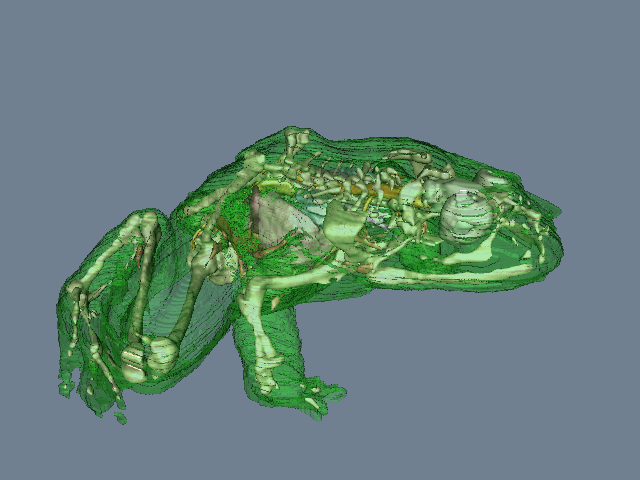
\includegraphics[width=\linewidth]{Figure12-9a}
		\caption{All frog parts and translucent skin.(\href{https://lorensen.github.io/VTKExamples/site/Cxx/Visualization/ViewFrogSkinAndTissue}{ViewFrogSkinAndTissue.cxx} or \href{https://lorensen.github.io/VTKExamples/site/Python/Visualization/ViewFrogSkinAndTissue/}{ViewFrogSkinAndTissue.py})}\label{fig:Figure12-9a}
	\end{subfigure}
	\hfill
	\begin{subfigure}[h]{0.48\linewidth}
		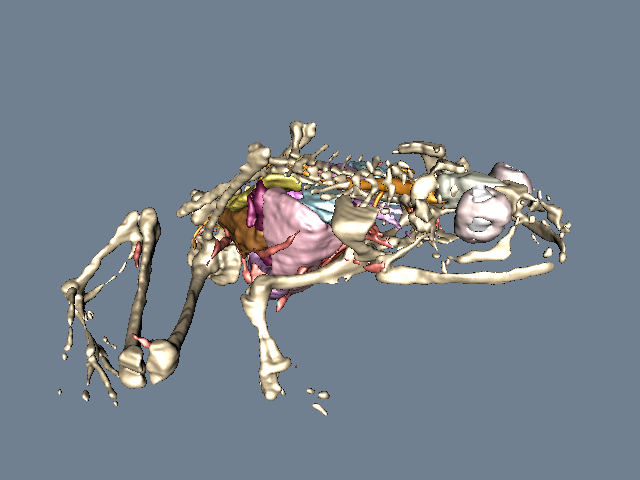
\includegraphics[width=\linewidth]{Figure12-9b}
		\caption{The complete frog without skin.(\href{https://lorensen.github.io/VTKExamples/site/Cxx/Visualization/ViewFrog}{ViewFrog.cxx} or \href{https://lorensen.github.io/VTKExamples/site/Python/Visualization/ViewFrog/}{ViewFrog.py})}\label{fig:Figure12-9b}
	\end{subfigure}%
	\hfill
	\begin{subfigure}[h]{0.48\linewidth}
		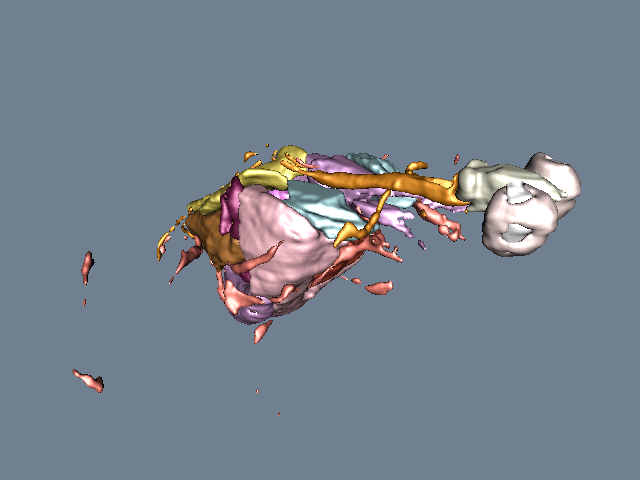
\includegraphics[width=\linewidth]{Figure12-9c}
		\caption{No skin or skeleton.(\href{https://lorensen.github.io/VTKExamples/site/Cxx/Visualization/ViewFrogA}{ViewFrogA.cxx} or \href{https://lorensen.github.io/VTKExamples/site/Python/Visualization/ViewFrogA/}{ViewFrogA.py})}\label{fig:Figure12-9c}
	\end{subfigure}
	\caption{Various frog images.}\label{fig:Figure12-9}
\end{figure}

Figure \ref{fig:Figure12-9} shows three views of the frog.

This lengthy example shows the power of a comprehensive visualization system like VTK.

\begin{itemize}

    \item We mixed image processing and computer graphics algorithms to process data created by an external segmentation process.

    \item We developed a generic approach that allows users to control the elements of the pipeline with a familiar scripting language, tcl.

    \item We separated the task into a ``batch'' portion and an ``interactive'' portion.

\end{itemize}

\subsection{Other Frog-Related Information}

The folks at Lawrence Berkeley National Laboratory have an impressive Web site that features the frog used in this example. The site describes how the frog data was obtained and also permits users to create mpeg movies of the frog. There are also other datasets available. Further details on ``The Whole Frog Project'' can be found at \href{http://www-itg.lbl.gov/Frog}{Frog}. Also, the Stanford University Medical Media and Information Technologies (SUMMIT) group has on-going work using the Berkeley frog. They are early VTK users. Enjoy their \emph{Virtual Creatures} project at: \href{http://summit.stanford.edu/creatures}{creatures}.
\index{applications!segmented volume data|)}\index{segmented volume data!application|)}\index{Tcl!application|)}

\section{Financial Visualization}
\index{applications!financial visualization|(}\index{financial visualization!application|(}\index{Tcl!application|(}

The application of 3D visualization techniques to financial data is relatively new. Historically, financial data has been represented using 2D plotting techniques such as line, scatter plots, bar charts, and pie charts. These techniques are especially well suited for the display of price and volume information for stocks, bonds, and mutual funds. Three--dimensional techniques are becoming more important due to the increased volume of information in recent years, and 3D graphics and visualization techniques are becoming interactive. Interactive rates mean that visualization can be applied to the day-to-day processing of data. Our belief is that this will allow deeper understanding of today's complex financial data and other more timely decisions.

In this example we go through the process of obtaining data, converting it to a form that we can use, and then using visualization techniques to view it. Some of the external software tools used in this example may be unfamiliar to you. This should not be a large concern. We have simply chosen the tools with which we are familiar. Where we have used an Awk script, you might choose to write a small C program to do the same thing. The value of the example lies in illustrating the high--level process of solving a visualization problem.

The first step is to obtain the data. We obtained our data from a public site on the World Wide Web (WWW) that archives stock prices and volumes for many publicly traded stocks. (This Web site has closed down since publication of the first edition. The data for this example are available on the CD--ROM.)

Once we have obtained the data, we convert it to a format that can be read into VTK. While VTK can read in a variety of data formats, frequently your data will not be in one of those. The data files we obtained are stored in the following format:

\begin{lstlisting}[numbers=none]
930830 49.375 48.812 49.250 1139.2 56.1056
930831 49.375 48.938 49.125 1360.4 66.8297
930902 49.188 48.688 48.750 1247.2 60.801
...
\end{lstlisting}

Each line stores the data for one day of trading. The first number is the date, stored as the last two digits of the year, followed by a two--digit month and finally the day of the month. The next three values represent the high, low, and closing price of the stock for that day. The next value is the volume of trading in thousands of shares. The final value is the volume of trading in millions of dollars.

We used an Awk\index{awk} script to convert the original data format into a VTK data file. (See the \emph{VTK User's Guide} for information on VTK file formats; or refer to the Web page \href{https://lorensen.github.io/VTKExamples/site/VTKFileFormats/}{VTKFileFormats}). This conversion could be done using many other approaches, such as writing a C program or a Tcl script.

\begin{lstlisting}[language=Awk, caption={Awk: converting data file to VTK.}]
BEGIN {print "\# vtk DataFile Version 2.0\\n
Data values for stock\nASCII\n\nDATASET POLYDATA"}
{count += 1}
{ d = $1%100}
{ m = int(($1%10000)/100)}
{ if (m == 2) d += 31}
{ if (m == 3) d += 59}
{ if (m == 4) d += 90}
{ if (m == 5) d += 120}
{ if (m == 6) d += 151}
{ if (m == 7) d += 181}
{ if (m == 8) d += 212}
{ if (m == 9) d += 243}
{ if (m == 10) d += 273}
{ if (m == 11) d += 304}
{ if (m == 12) d += 334}
{ d = d + (int($1/10000) - 93)*365}
{dates[count] = d; prices[count] = $4; volumes[count] = $5}
END {
  print "POINTS " count " float";
  for (i = 1; i \<= count; i++) print dates[i] " " prices[i] " 0 ";
  print "\nLINES 1 " (count + 1) " " count;
  for (i = 0; i \< count; i++) print i;
  print "\nPOINT\_DATA " count "\nSCALARS volume float";
  print "LOOKUP\_TABLE default";
  for (i = 1; i \<= count; i++) print volumes[i];
  }
\end{lstlisting}

The above Awk script performs the conversion. Its first line outputs the required header information indicating that the file is a VTK data file containing polygonal data. It also includes a comment indicating that the data represents stock values. There are a few different VTK data formats that we could have selected. It is up to you to decide which format best suits the data you are visualizing. We have judged the polygonal format ( vtkPolyData ) as best suited for this particular stock visualization.

The next line of the Awk script creates a variable named count that keeps track of how many days worth of information is in the file. This is equivalent to the number of lines in the original data file.

The next fourteen lines convert the six digit date into a more useful format, since the original format has a number of problems. If we were to blindly use the original format and plot the data using the date as the independent variable, there would be large gaps in our plot. For example,  $931231$ is the last day of $1993$ and $940101$ is the first day of $1994$. Chronologically, these two dates are sequential, but mathematically there are $(940101 - 931231 = 8870$ values between them. A simple solution would be to use the line number as our independent variable. This would work as long as we knew that every trading day was recorded in the data file. It would not properly handle the situation where the market was open, but for some reason data was not recorded. A better solution is to convert the dates into numerically ordered days. The preceding Awk script sets January 1, 1993, as day number one, and then numbers all the following days from there. At the end of these $14$ lines the variable, d, will contain the resulting value.

The next line in our Awk script stores the converted date, closing price, and dollar volume  into arrays indexed by the line number stored in the variable count. Once all the lines have been read and stored into the arrays, we write out the rest of the VTK data file. We have selected the date as our independent variable and \emph{x} coordinate. The closing price we store as the \emph{y} coordinate, and the \emph{z} coordinate we set to zero. After indicating the number and type of points to be stored, the Awk script loops through all the points and writes them out to the VTK data file. It then writes out the line connectivity list. In this case we just connect one point to the next to form a polyline for each stock. Finally, we write out the volume information as scalar data associated with the points. Portions of the resulting VTK data file are shown below.

\begin{lstlisting}[numbers=none]
# vtk DataFile Version 2.0 Data values for stock
ASCII
DATASET POLYDATA
POINTS 348 float
242 49.250 0
243 49.125 0
245 48.750 0
246 48.625 0
...
LINES 1 349 348
0
1
2
3
...
POINT_DATA 348
SCALARS volume float
LOOKUP_TABLE default
1139.2
1360.4
1247.2
1745.4
...
\end{lstlisting}

Now that we have generated the VTK data file, we can start the process of creating a visualization for the stock data. To do this, we wrote a Tcl script to be used with the Tcl--based VTK executable. At a high level the script reads in the stock data, sends it through a tube filter, creates a label for it, and then creates an outline around the resulting dataset. Ideally, we would like to display multiple stocks in the same window. To facilitate this, we designed the Tcl script to use a procedure to perform operations on a per stock basis. The resulting script is listed below.


\begin{lstlisting}[language=TCL, caption={Tcl script for stock case study.}, escapechar=\%]
package require vtk
#  this is a tcl script for the stock case study
#  Create the RenderWindow, Renderer and both Actors vtkRenderer ren1
vtkRenderWindow renWin
  renWin AddRenderer ren1
vtkRenderWindowInteractor iren
  iren SetRenderWindow renWin

# create the outline
vtkAppendPolyData%\index{vtkAppendPolyData!application}% apf
vtkOutlineFilter olf
  olf SetInputConnection [apf GetOutputPort]
vtkPolyDataMapper outlineMapper
  outlineMapper SetInputConnection [olf GetOutputPort]
vtkActor outlineActor
  outlineActor SetMapper outlineMapper

set zpos 0
# create the stocks
proc AddStock {prefix name x y z} {
  global zpos

  # create labels
  vtkTextSource $prefix.TextSrc
    $prefix.TextSrc SetText "$name"
    $prefix.TextSrc SetBacking 0
  vtkPolyDataMapper $prefix.LabelMapper
    $prefix.LabelMapper SetInput [$prefix.TextSrc GetOutput]
  vtkFollower%\index{vtkFollower!example}% $prefix.LabelActor
    $prefix.LabelActor SetMapper $prefix.LabelMapper
    $prefix.LabelActor SetPosition $x $y $z
    $prefix.LabelActor SetScale 0.25 0.25 0.25
    eval $prefix.LabelActor SetOrigin
        [$prefix.LabelMapper GetCenter]
  #  create a sphere source and actor
  vtkPolyDataReader $prefix.PolyDataRead
    $prefix.PolyDataRead SetFileName
		"../../../vtkdata/$prefix.vtk"
  vtkTubeFilter $prefix.TubeFilter
    $prefix.TubeFilter
    SetInputConnection \
        [$prefix.PolyDataRead GetOutputPort]
	$prefix.TubeFilter SetNumberOfSides 8
	$prefix.TubeFilter SetRadius 0.5
    $prefix.TubeFilter SetRadiusFactor 10000
  vtkTransform $prefix.Transform
	$prefix.Transform Translate 0 0 $zpos
	$prefix.Transform Scale 0.15 1 1
  vtkTransformPolyDataFilter $prefix.TransformFilter
    $prefix.TransformFilter SetInputConnection
        [$prefix.TubeFilter GetOutputPort]
    $prefix.TransformFilter SetTransform
    $prefix.Transform
  # increment zpos
  set zpos [expr $zpos + 10]
  vtkPolyDataMapper $prefix.StockMapper
    $prefix.StockMapper SetInputConnection
        [$prefix.TransformFilter GetOutputPort]
  vtkActor $prefix.StockActor
    $prefix.StockActor SetMapper $prefix.StockMapper
    $prefix.StockMapper SetScalarRange 0 8000
    [$prefix.StockActor GetProperty] SetAmbient 0.5
    [$prefix.StockActor GetProperty] SetDiffuse 0.5

  apf AddInput [$prefix.TransformFilter GetOutput]

  ren1 AddActor $prefix.StockActor
  ren1 AddActor $prefix.LabelActor
  $prefix.LabelActor SetCamera [ren1 GetActiveCamera]
}

#  set up the stocks
ddStock GE "GE" 94 46 4
AddStock GM "GM" 107 39 14
AddStock IBM "IBM" 92 70 16
AddStock DEC "DEC" 70 19 26

#  Add the actors to the renderer, set the background and size
#
ren1 AddActor outlineActor
ren1 SetBackground 0.1 0.2 0.4
renWin SetSize 1200 600

#  render the image
[ren1 GetActiveCamera] SetViewAngle 10
ren1 ResetCamera
[ren1 GetActiveCamera] Zoom 2.8
[ren1 GetActiveCamera] Elevation 90
[ren1 GetActiveCamera] SetViewUp 0 0 -1
iren Initialize

#  prevent the tk window from showing up then start the event loop
wm withdraw .
\end{lstlisting}

The first part of this script consists of the standard procedure for renderer and interactor creation that can be found in almost all of the VTK Tcl scripts. The next section creates the objects necessary for drawing an outline around all of the stock data. A vtkAppendPolyData filter is used to append all of the stock data together. This is then sent through a vtkOutlineFilter to create a bounding box around the data. A mapper and actor are created to display the result.

In the next part of this script, we define the procedure to add stock data to this visualization. The procedure takes five arguments: the name of the stock, the label we want displayed, and the x, y, z coordinates defining where to position the label. The first line of the procedure indicates that the variable ren1 should be visible to this procedure. By default the procedure can only access its own local variables. Next, we create the label using a vtkTextSource, vtkPolyDataMapper, and vtkFollower\index{vtkFollower}. The names of these objects are all prepended with the variable ``\$prefix.'' so that the instance names will be unique. An instance of vtkFollower is used instead of the usual vtkActor\index{vtkActor}, because we always want the text to be right--side up and facing the camera. The vtkFollower class provides this functionality. The remaining lines position and scale the label appropriately. We set the origin of the label to the center of its data. This insures that the follower will rotate about its center point.

The next group of lines creates the required objects to read in the data, pass it through a tube filter and a transform filter, and finally display the result. The tube filter uses the scalar data (stock volume in this example) to determine the radius of the tube. The mapper also uses the scalar data to determine the coloring of the tube. The transform filter uses a transform object to set the stock's position based on the value of the variable zpos. For each stock, we will increment zpos by 10, effectively shifting the next stock over 10 units from the current stock. This prevents the stocks from being stacked on top of each other. We also use the transform to compress the x--axis to make the data easier to view. Next, we add this stock as an input to the append filter and add the actors and followers to the renderer. The last line of the procedure sets the follower's camera to be the active camera of the renderer.

Back in the main body of the Tcl script, we invoke the AddStock procedure four times with four different stocks. Finally, we add the outline actor and customize the renderer and camera to  four different stocks. Finally, we add the outline actor and customize the renderer and camera to produce a nice initial view.

Two different views of the result are displayed in Figure \ref{fig:Figure12-10}. The top image shows a history of stock closing prices for our four stocks. The color and width of these lines correspond to the volume of the stock on that day. The lower image more clearly illustrates the changes in stock volume by looking at the data from above.

\begin{figure}[!htb]
	\centering
	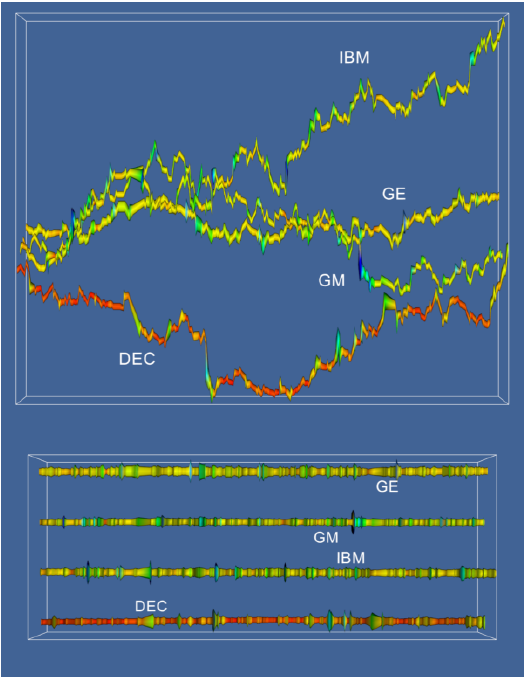
\includegraphics[width=0.74\linewidth]{Figure12-10}
	\caption{Two views from the stock visualization script. The top shows closing price over time; the bottom shows volume over time ( stocks.tcl ).}
	\label{fig:Figure12-10}
\end{figure}

\begin{figure}[!htb]
	\centering
	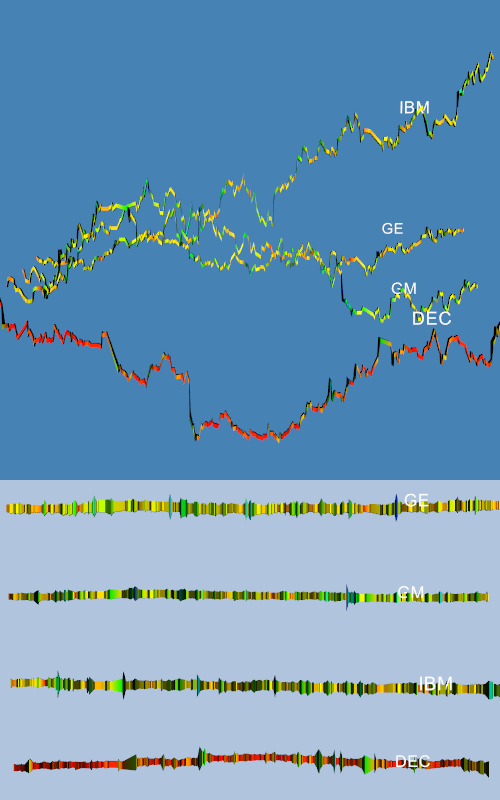
\includegraphics[width=0.74\linewidth]{Figure12-11}
	\caption{Two more views of the stock case study. Here the
		tube filter has been replaced by a ribbon filter followed with a
		linear extrusion filter.(\href{https://lorensen.github.io/VTKExamples/site/Cxx/VisualizationAlgorithms/Stocks/}{Stocks.cxx}) or (\href{https://lorensen.github.io/VTKExamples/site/Python//VisualizationAlgorithms/Stocks/}{Stocks.py})}
	\label{fig:Figure12-11}
\end{figure}

A legitimate complaint with Figure \ref{fig:Figure12-10} is that the changing
width of the tube makes it more difficult to see the true shape of the
price verses the time curve. We can solve this problem by using a
ribbon filter followed by a linear extrusion filter, instead of the
tube filter. The ribbon filter will create a ribbon whose width will
vary in proportion to the scalar value of the data. We then use

the linear extrusion filter to extrude this ribbon along the \emph{y}-axis
so that it has a constant thickness.

The resulting views are shown in Figure \ref{fig:Figure12-11}.
\index{applications!financial visualization|)}\index{financial visualization!application|)}\index{Tcl!application|)}

\section{Implicit Modelling}
\index{applications!implicit modelling|(}\index{C++!application|(}\index{implicit modelling!application|(}

The \emph{Visualization Toolkit} has some useful geometric modelling capabilities. One of the most powerful features is implicit modelling. In this example we show how to use polygonal descriptions of objects and create `blobby'' models of them using the implicit modelling objects in VTK. This example generates a logo for the \emph{Visualization Toolkit} from polygonal representations of the letters \emph{v}, \emph{t}, and \emph{k}.

\begin{figure}[!htb]
	\centering
	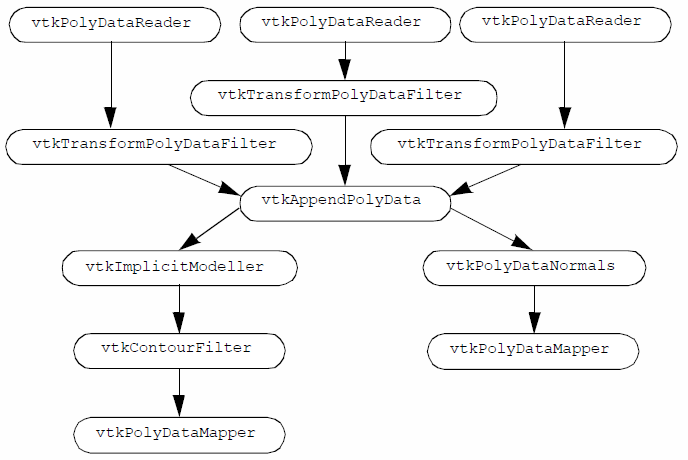
\includegraphics[width=0.8\textwidth]{Figure12-12}
	\caption{The visualization pipeline for the VTK blobby logo.}
	\label{fig:Figure12-12}
\end{figure}

We create three separate visualization pipelines, one for each letter. Figure \ref{fig:Figure12-12} shows the visualization pipeline. As is common in VTK applications, we design a pipeline and fill in the details of the instance variables just before we render. We pass the letters through a vtkTransformPolyDataFilter to position them relative to each other. Then we combine all of the polygons from the transformed letters into one polygon dataset using the vtkAppendPolyData\index{vtkAppendPolyData} filter. The vtkImplicitModeller creates a volume dataset of dimension $64^3$ with each voxel containing a scalar value that is the distance to the nearest polygon. Recall from ``Implicit Modelling'' on page \pageref{subsec:implicit_modelling} that the implicit modelling algorithm lets us specify the region of influence of each polygon. Here we specify this using the SetMaximumDistance() method of the vtkImplicitModeller. By restricting the region of influence, we can significantly improve performance of the implicit modelling algorithm. Then we use vtkContourFilter\index{vtkContourFilter!application} to extract an isosurface\index{isosurface!application} that approximates a distance of 1.0 from each polygon. We create two actors: one for the blobby logo and one for the original polygon letters. Notice that both actors share the polygon data created by vtkAppendPolyData. Because of the nature of the VTK visualization pipeline (see ``Implicit Execution'' on page \pageref{subsec:implicit_execution} ), the appended data will only be created once by the portion of the pipeline that is executed first. As a final touch, we move the polygonal logo in front of the blobby logo. Now we will go through the example in detail.

First, we read the geometry files that contain polygonal models of each letter in the logo. The data is in VTK polygonal format, so we use vtkPolyDataReader.

\begin{lstlisting}[language=C++, caption={Reading the polygonal models of each letter.}]
vtkPolyDataReader *letterV = vtkPolyDataReader::New();
  letterV->SetFileName ("v.vtk");

vtkPolyDataReader *letterT = vtkPolyDataReader::New();
  letterT->SetFileName ("t.vtk");

vtkPolyDataReader *letterK = vtkPolyDataReader::New();
  letterK->SetFileName ("k.vtk");
\end{lstlisting}

We want to transform each letter into its appropriate location and orientation within the logo. We create the transform filters here, but defer specifying the location and orientation until later in the program.

\begin{lstlisting}[language=C++, caption={Transform each letter into ita appropriate location.}]
vtkTransform *VTransform = vtkTransform::New();
  vtkTransformPolyDataFilter *VTransformFilter =
  vtkTransformPolyDataFilter::New();

VTransformFilter->SetInputConnection (letterV->GetOutputPort());
  VTransformFilter->SetTransform (VTransform);

vtkTransform *TTransform = vtkTransform::New();
  vtkTransformPolyDataFilter *TTransformFilter =
  vtkTransformPolyDataFilter::New();

TTransformFilter->SetInputConnection (letterT->GetOutputPort());
  TTransformFilter->SetTransform (TTransform);

vtkTransform *KTransform = vtkTransform::New();
  vtkTransformPolyDataFilter *KTransformFilter =
  vtkTransformPolyDataFilter::New();

  KTransformFilter->SetInputConnection (letterK->GetOutputPort());
  KTransformFilter->SetTransform (KTransform);
\end{lstlisting}

We collect all of the transformed letters into one set of polygons by using an instance of the class vtkAppendPolyData.

\begin{lstlisting}[language=C++, caption={Collect the transformed letters into one set of polygons.}]
vtkAppendPolyData *appendAll = vtkAppendPolyData::New();
  appendAll->AddInputConnection (VTransformFilter->GetOutputPort());
  appendAll->AddInputConnection (TTransformFilter->GetOutputPort());
  appendAll->AddInputConnection (KTransformFilter->GetOutputPort());
\end{lstlisting}

Since the geometry for each letter did not have surface normals, we add them here. We use vtkPolyDataNormals. Then we complete this portion of the pipeline by creating a mapper and an actor.

\begin{lstlisting}[language=C++, caption={Add surface normals and create mapper and actor.}]
// create normals
vtkPolyDataNormals *logoNormals = vtkPolyDataNormals::New();
  logoNormals->SetInputConnection (appendAll->GetOutputPort());
  logoNormals->SetFeatureAngle (60);

// map to rendering primitives
vtkPolyDataMapper *logoMapper = vtkPolyDataMapper::New();
  logoMapper->SetInputConnection (logoNormals->GetOutputPort());

// now an actor
vtkActor *logo = vtkActor::New();
  logo->SetMapper (logoMapper);
\end{lstlisting}

We create the blobby logo with the implicit modeller, and then extract the logo with vtkContourFilter. The pipeline is completed by creating a mapper and an actor.

\begin{lstlisting}[language=C++, caption={Create an implicit model of the letters and extract the logo.}, escapechar=\$]
// now create an implicit model of the letters
vtkImplicitModeller$\index{vtkImplicitModeller!application}$ *blobbyLogoImp = vtkImplicitModeller::New();
  blobbyLogoImp->SetInputConnection (appendAll->GetOutputPort());
  blobbyLogoImp->SetMaximumDistance (.075);
  blobbyLogoImp->SetSampleDimensions (64,64,64);
  blobbyLogoImp->SetAdjustDistance (0.05);

// extract an iso surface
vtkContourFilter *blobbyLogoIso = vtkContourFilter::New();
  blobbyLogoIso->SetInputConnection (blobbyLogoImp->GetOutputPort());
  blobbyLogoIso->SetValue (1, 1.5);

// map to rendering primitives
vtkPolyDataMapper *blobbyLogoMapper = vtkPolyDataMapper::New();
  blobbyLogoMapper->SetInputConnection (blobbyLogoIso->GetOutputPort());
  blobbyLogoMapper->ScalarVisibilityOff ();

// now an actor
vtkActor *blobbyLogo = vtkActor::New();
  blobbyLogo->SetMapper(blobbyLogoMapper);
  blobbyLogo->SetProperty(banana);
\end{lstlisting}

To improve the look of our resulting visualization, we define a couple of organic colors. Softer colors show up better on some electronic media (e.g., VHS video tape) and are pleasing to the eye.

\begin{lstlisting}[language=C++, caption={Define colors.}]
vtkProperty *tomato = vtkProperty::New();
  tomato->SetDiffuseColor(1, 0.3882, 0.2784);
  tomato->SetSpecular(0.3);
  tomato->SetSpecularPower(20);
vtkProperty *banana = vtkProperty::New();
  banana->SetDiffuseColor(0.89, 0.81, 0.34);
  banana->SetDiffuse (0.7);
  banana->SetSpecular(0.4);
  banana->SetSpecularPower(20);
\end{lstlisting}

These colors are then assigned to the appropriate actors.

\begin{lstlisting}[language=C++, caption={Assign colors to the appropriate actors.}]
  logo->SetProperty(tomato);
  blobbyLogo->SetProperty(banana);
\end{lstlisting}

And finally, we position the letters in the logo and move the
polygonal logo out in front of the blobby logo by modifying the
actor's position.

\begin{lstlisting}[language=C++, caption={Position the letters and move the polygonal logo.}]
  VTransform->Translate (-16,0,12.5);
  VTransform->RotateY (40);
  KTransform->Translate (14, 0, 0);
  KTransform->RotateY (-40);

  // move the polygonal letters to the front
  logo->SetPosition(0,0,6);
\end{lstlisting}

\begin{figure}[htb]
	\begin{subfigure}[h]{0.48\linewidth}
		
\includegraphics[width=0.96\linewidth]{Figure12-13a}
		\caption*{}
		\label{fig:Figure12-13a}
	\end{subfigure}
	\hfill
	\begin{subfigure}[h]{0.48\linewidth}
		
\includegraphics[width=0.96\linewidth]{Figure12-13b}
		\caption*{}
		\label{fig:Figure12-13b}
	\end{subfigure}
	\caption{A logo created with vtkImplicitModeller.(\href{https://lorensen.github.io/VTKExamples/site/Cxx/Visualization/BlobbyLogo/}{BlobbyLogo.cxx}) or (\href{https://lorensen.github.io/VTKExamples/site/Python/Visualization/BlobbyLogo/}{BlobbyLogo.py})}\label{fig:Figure12-13}
\end{figure}


An image made from the techniques described in this section is shown
in Figure \ref{fig:Figure12-13}  Note that the image on the left has been augmented with a texture map.
\index{applications!implicit modelling|)}\index{C++!application|)}\index{implicit modelling!application|)}

\section{Computational Fluid Dynamics}
\index{applications!computational fluid dynamics|(}\index{computational fluid dynamics!application|(}\index{finite difference method!application|(}

Computational Fluid Dynamics (CFD) visualization poses a challenge to any visualization toolkit. CFD studies the flow of fluids in and around complex structures. Often, large amounts of super--computer time is used to derive scalar and vector data in the flow field. Since CFD computations produce multiple scalar and vector data types, we will apply many of the tools described in this book. The challenge is to combine multiple representations into meaningful visualizations that extract information without overwhelming the user.

CFD analysts often employ finite difference grids. A finite difference grid represents the discretization of the problem domain into small computational cells. The grid allows the analyst to create a large system of equations that can then be solved on a computer.
The grid is topologically uniform in \emph{i--j--k} space, but the corresponding physical coordinates need not be uniformly distributed. This is what we call a structured grid dataset in VTK.

There are a number of techniques we can use when we first look at the complex data presented by CFD applications. Since we need to apply several algorithms to the data, and since there will be many parameter changes for these algorithms, we suggest using the Tcl interpreter rather than C++ code. Our strategy for visualizing this CFD data includes the following:

\begin{itemize}

    \item Display the computational grid. The analyst carefully constructed the finite difference grid to have a higher density in regions where rapid changes occur in the flow variables. We will display the grid in wireframe so we can see the computational cells.

    \item Display the scalar fields on the computational grid. This will give us an overview of where the scalar data is changing. We will experiment with the extents of the grid extraction to focus on interesting areas.

    \item Explore the vector field by seeding streamlines with a spherical cloud of points. Move the sphere through areas of rapidly changing velocity.

    \item Try using the computational grid itself as seeds for the streamlines. Of course we will have to restrict the extent of the grid you use for this purpose. Using the grid, we will be able to place more seeds in regions where the analyst expected more action.

\end{itemize}

For this case study, we use a dataset from NASA called the LOx Post. It simulates the flow of liquid oxygen across a flat plate with a cylindrical post perpendicular to the flow \cite{Rogers86}. This analysis models the flow in a rocket engine. The post promotes mixing of the liquid oxygen.

We start by exploring the scalar and vector fields in the data. By calculating the magnitude of the velocity vectors, we derive a scalar field. This study has a particularly interesting vector field around the post. We seed the field with multiple starting points (using points arranged along a curve, referred to as a \emph{rake}) and experiment with parameters for the streamlines. Streampolygons\index{streampolygon} are particularly appropriate here and do a nice job of showing the flow downstream from the post. We animate the streamline creation by moving the seeding line or rake back and forth behind the post.

\begin{figure}[htb]
	\begin{subfigure}[h]{0.48\linewidth}
		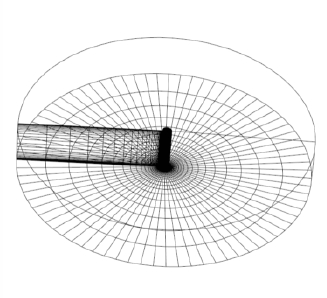
\includegraphics[width=0.96\linewidth]{Figure12-14a}
		\caption*{}
		\label{fig:Figure12-14a}
	\end{subfigure}
	\hfill
	\begin{subfigure}[h]{0.48\linewidth}
		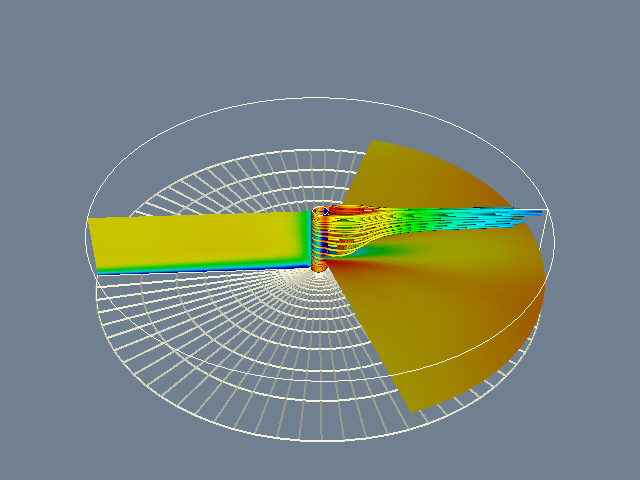
\includegraphics[width=0.96\linewidth]{Figure12-14b}
		\caption*{}
		\label{fig:Figure12-14b}
	\end{subfigure}
	\caption{Portion of computational grid for the LOx post.(\href{https://lorensen.github.io/VTKExamples/site/Cxx/VisualizationAlgorithms/LOxGrid/}{LOxGrid.cxx}) or (\href{https://lorensen.github.io/VTKExamples/site/Python/VisualizationAlgorithms/LOxGrid/}{LOxGrid.py})}\label{fig:Figure12-14}
\end{figure}

Following our own advice, we first display the computational grid. The
following Tcl code produced the left image of Figure \ref{fig:Figure12-14}.

\begin{lstlisting}[language=TCL, caption={Display the computational grid.}]
# read data
vtkPLOT3DReader pl3d
  pl3d SetXYZFileName "$env(VTK_TEXTBOOK_DATA)/postxyz.bin"
  pl3d SetQFileName "$env(VTK_TEXTBOOK_DATA)/postq.bin"
  pl3d IBlankingOn
  pl3d Update
# computational planes: the floor
vtkStructuredGridGeometryFilter floorComp
  floorComp SetExtent 0 37 0 75 0 0
  floorComp SetInputConnection [pl3d GetOutputPort]
vtkPolyDataMapper floorMapper
  floorMapper SetInputConnection [floorComp GetOutputPort]
  floorMapper ScalarVisibilityOff
vtkActor floorActor
  floorActor SetMapper floorMapper
  [floorActor GetProperty] SetColor 0 0 0
  [floorActor GetProperty] SetRepresentationToWireframe
# the post
vtkStructuredGridGeometryFilter postComp
  postComp SetExtent 10 10 0 75 0 37
  postComp SetInputConnection [pl3d GetOutputPort]
vtkPolyDataMapper postMapper
  postMapper SetInputConnection [postComp GetOutputPort]
  postMapper ScalarVisibilityOff
vtkActor postActor
  postActor SetMapper postMapper
  [postActor GetProperty] SetColor 0 0 0
  [postActor GetProperty] SetRepresentationToWireframe
# plane upstream of the flow
vtkStructuredGridGeometryFilter fanComp
  fanComp SetExtent 0 37 38 38 0 37
  fanComp SetInputConnection [pl3d GetOutputPort]
vtkPolyDataMapper fanMapper
  fanMapper SetInputConnection [fanComp GetOutputPort]
  fanMapper ScalarVisibilityOff
vtkActor fanActor
  fanActor SetMapper fanMapper
  [fanActor GetProperty] SetColor 0 0 0
  [fanActor GetProperty] SetRepresentationToWireframe
# outline
vtkStructuredGridOutlineFilter outline
  outline SetInputConnection [pl3d GetOutputPort]
vtkPolyDataMapper outlineMapper
  outlineMapper SetInputConnection [outline GetOutputPort]
vtkActor outlineActor
  outlineActor SetMapper outlineMapper
  [outlineActor GetProperty] SetColor 0 0 0
# Create graphics stuff
vtkRenderer ren1
vtkRenderWindow renWin
  renWin AddRenderer ren1
vtkRenderWindowInteractor iren
  iren SetRenderWindow renWin
# Add the actors to the renderer, set the background and size
#
  ren1 AddActor outlineActor
  ren1 AddActor floorActor
  ren1 AddActor postActor
  ren1 AddActor fanAct
\end{lstlisting}

To display the scalar field using color mapping\index{color mapping!application}, we must change the actor's representation from wireframe to surface, turn on scalar visibility for each vtkPolyDataMapper, set each mapper's scalar range, and render again, producing the right image of Figure \ref{fig:Figure12-14}.

\begin{lstlisting}[language=TCL, caption={Dicplay the scalar field.}]
  postActor SetRepresentationToSurface
  fanActor SetRepresentationToSurface
  floorActor SetRepresentationToSurface
  postMapper ScalarVisibilityOn
  postMapper SetScalarRange [[pl3d GetOutput] GetScalarRange]
  fanMapper ScalarVisibilityOn
  fanMapper SetScalarRange [[pl3d GetOutput] GetScalarRange]
  floorMapper ScalarVisibilityOn
  floorMapper SetScalarRange [[pl3d GetOutput] GetScalarRange]
\end{lstlisting}

\begin{figure}[!htb]
	\centering
	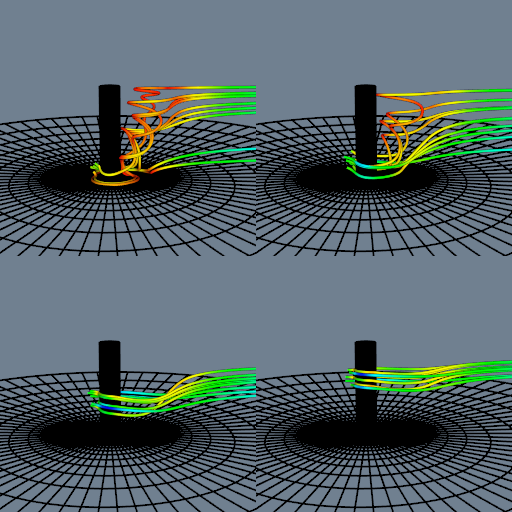
\includegraphics[width=0.8\textwidth]{Figure12-15}
	\caption{Streamlines seeded with spherical cloud of points. Four separate cloud positions are shown.(\href{https://lorensen.github.io/VTKExamples/site/Cxx/VisualizationAlgorithms/LOxSeeds/}{LOxSeeds.cxx}) or (\href{https://lorensen.github.io/VTKExamples/site/Python/VisualizationAlgorithms/LOxSeeds/}{LOxSeeds.py})}
	\label{fig:Figure12-15}
\end{figure}


Now, we explore the vector field using vtkPointSource. Recall that this object generates a random cloud of points around a spherical center point. We will use this cloud of points to generate stream-lines. We place the center of the cloud near the post since this is where the velocity seems to be changing most rapidly. During this exploration, we use streamlines\index{streamline!application} rather than streamtubes for reasons of efficiency. The Tcl code is as follows.

\begin{lstlisting}[language=TCL, caption={Explore the vector field using a point source.}]
# spherical seed points
vtkPointSource rake
  rake SetCenter -0.74 0 0.3
  rake SetNumberOfPoints 10
vtkStreamLine streamers
  streamers SetInputConnection [pl3d GetOutputPort]
  streamers SetSourceConnection [rake GetOutputPort]
  streamers SetMaximumPropagationTime 250
  streamers SpeedScalarsOn
  streamers SetIntegrationStepLength 0.2
  streamers SetStepLength 0.25
vtkPolyDataMapper mapTubes
  mapTubes SetInputConnection [streamers GetOutputPort]
  eval mapTubes SetScalarRange [[pl3d GetOutput] GetScalarRange]
vtkActor tubesActor
  tubesActor SetMapper mapTubes
\end{lstlisting}

Figure \ref{fig:Figure12-15} shows streamlines seeded\index{streamline!seeding} from four locations along the post.
Notice how the structure of the flow begins to emerge as the starting positions for the streamlines are moved up and down in front of the post. This is particularly true if we do this interactively; the mind assembles the behavior of the streamlines into a global understanding of the flow field.

\begin{figure}[!htb]
	\centering
	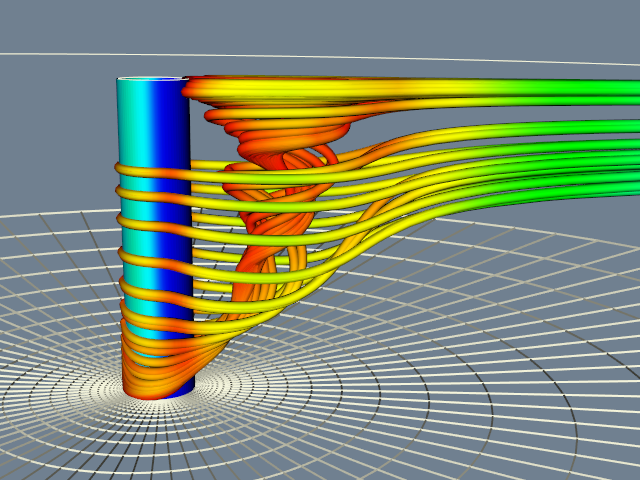
\includegraphics[width=0.8\textwidth]{Figure12-16}
	\caption{Streamlines seeded with spherical cloud of points. Four separate cloud positions are shown.(\href{https://lorensen.github.io/VTKExamples/site/Cxx/VisualizationAlgorithms/LOx/}{LOx.cxx}) or (\href{https://lorensen.github.io/VTKExamples/site/Python/VisualizationAlgorithms/LOx/}{LOx.py})}
	\label{fig:Figure12-16}
\end{figure}

For a final example, we use the computational grid to seed streamlines and then generate streamtubes as is shown in Figure \ref{fig:Figure12-16}. A nice feature of this approach is that we generate more streamlines in regions where the analyst constructed a denser grid. The only change we need to make is to replace the rake from the sphere source with a portion of the grid geometry.

\begin{lstlisting}[language=TCL, caption={Use the computational grid to seed streamlines and then generate streamtubes.}]
vtkStructuredGridGeometryFilter seedsComp
  seedsComp SetExtent 10 10 37 39 1 35
  seedsComp SetInput [pl3d GetOutput]
  streamers SetSourceConnection [seedsComp GetOutputPort]
# create tubes
vtkTubeFilter tubes
  tubes SetInputConnection [streamers GetOutputPort]
  tubes SetNumberOfSides 8
  tubes SetRadius 0.08
  tubes SetVaryRadiusOff
# change input to streamtubes
  mapTubes SetInputConnection [tubes GetOutputPort]
\end{lstlisting}

There are a number of other methods we could use to visualize this data. A 3D widget such as the vtkLineWidget could be used to seed the streamlines interactively (see ``3D Widgets and User Interaction'' on page \pageref{sec:3D_widgets_user_interaction}). As we saw in ``Point Probe'' on page \pageref{subsec:examples.point_probe}, probing the data
for numerical values is a valuable technique. In particular, if the probe is a line we can use it in combination with vtkXYPlotActor to graph the variation of data value along the line. Another useful visualization would be to identify regions of vorticity. We could use Equation \ref{eq:9.12} in conjunction with an isocontouring algorithm (e.g., vtkContourFilter ) to creates isosurfaces of large helical--density. \index{applications!computational fluid dynamics|)}\index{computational fluid dynamics!application|)}\index{finite difference method!application|)}

\section{Finite Element Analysis}
\index{applications!finite element method|(}\index{finite element method!application|(}

Finite element analysis is a widely used numerical technique for finding solutions of partial differential equations. Applications of finite element analysis include linear and nonlinear structural, thermal, dynamic, electromagnetic, and flow analysis. In this application we will visualize the results of a blow molding process.

\begin{figure}[!htb]
	\centering
	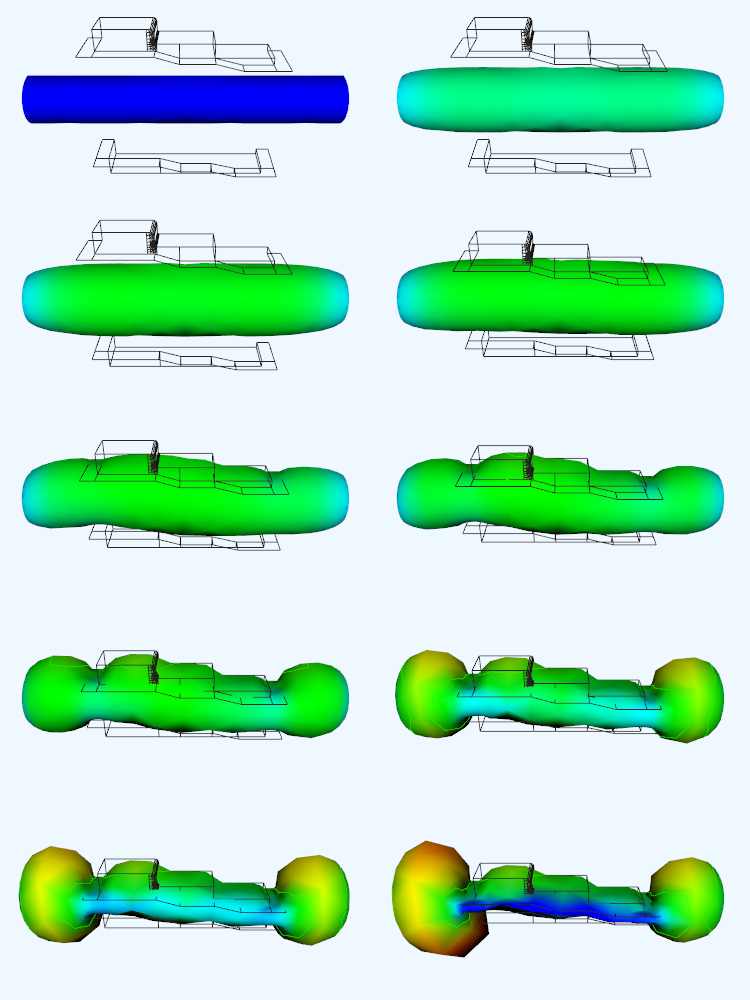
\includegraphics[width=0.8\textwidth]{Figure12-17}
	\caption{Ten frames from a blow molding finite element analysis. Mold halves (shown in wireframe) are closed around a parison as the parison is inflated. Coloring indicates thickness --- red areas are thinner than blue.(\href{https://lorensen.github.io/VTKExamples/site/Cxx/Visualization/Blow/}{Blow.cxx}) or (\href{https://lorensen.github.io/VTKExamples/site/Python/Visualization/Blow/}{Blow.py})}
	\label{fig:Figure12-17}
\end{figure}

In the extrusion blow molding process, a material is extruded through an annular die to form a hollow cylinder. This cylinder is called a \emph{parison}. Two mold halves are then closed on the parison, while at the same time the parison is inflated with air. Some of the parison material remains within the mold while some becomes waste material. The material is typically a polymer plastic softened with heat, but blow molding has been used to form metal parts. Plastic bottles are often manufactured using a blow molding process.

Designing the parison die and molds is not easy. Improper design results in large variations in the wall thickness. In some cases the part may fail in thin--walled regions. As a result, analysis tools based on finite element techniques have been developed to assist in the design of molds and dies.

The results of one such analysis are shown in Figure \ref{fig:Figure12-17}. The polymer was molded using an isothermal, nonlinear-elastic, incompressible (rubber--like) material. Triangular membrane finite elements were used to model the parison, while a combination of triangular and quadrilateral finite elements were used to model the mold. The mold surface is assumed to be rigid, and the parison is assumed to attach to the mold upon contact. Thus the thinning of the parison is controlled by its stretching during inflation and the sequence in which it contacts the mold.

Figure \ref{fig:Figure12-17} illustrates 10 steps of one analysis. The color of the parison indicates its thickness. Using a rainbow scale, red areas are thinnest while blue regions are thickest. Our visualization shows
clearly one problem with the analysis technique we are using. Note that while the nodes (i.e., points) of the finite element mesh are prevented from passing through the mold, the interior of the triangular elements are not. This is apparent from the occlusion of the mold wireframe by the parison mesh.

\begin{figure}[!htb]
	\centering
	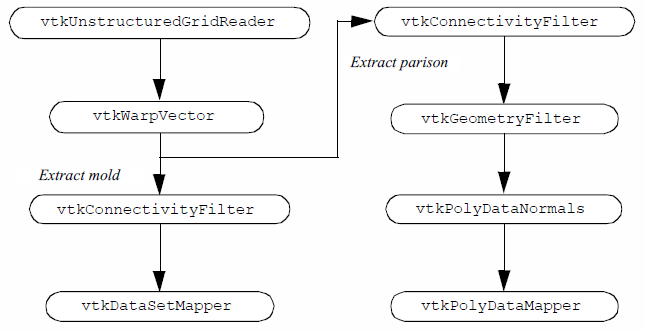
\includegraphics[width=0.8\textwidth]{Figure12-18}
	\caption{The network topology for the generation of the blow molding image.}
	\label{fig:Figure12-18}
\end{figure}

The network topology used to generate these images is shown in Figure \ref{fig:Figure12-18} with the corresponding Tcl script shown below

\begin{lstlisting}[language=TCL, caption={Script to generate the blow molding image.}]
# Create blow molding image (datapoint 5)
package require vtk
package require vtkinteraction

# Create graphics stuff
vtkRenderer ren1
vtkRenderWindow renWin
  renWin AddRenderer ren1
vtkRenderWindowInteractor iren
  iren SetRenderWindow renWin

# create reader and warp data with vectors
vtkUnstructuredGridReader reader
  reader SetFileName "$VTK_DATA_ROOT/Data/blow.vtk"
  reader SetScalarsName "thickness9"
  reader SetVectorsName "displacement9"
vtkWarpVector warp
  warp SetInputConnection [reader GetOutputPort]

# extract mold from mesh using connectivity
vtkConnectivityFilter connect
  connect SetInputConnection [warp GetOutputPort]
  connect SetExtractionModeToSpecifiedRegions
  connect AddSpecifiedRegion 0
  connect AddSpecifiedRegion 1
vtkDataSetMapper moldMapper
  moldMapper SetInputConnection [connect GetOutputPort]
  moldMapper ScalarVisibilityOff
vtkActor moldActor
  moldActor SetMapper moldMapper
  [moldActor GetProperty] SetColor .2 .2 .2
  [moldActor GetProperty] SetRepresentationToWireframe

# extract parison from mesh using connectivity
vtkConnectivityFilter connect2
  connect2 SetInputConnection [warp GetOutputPort]
  connect2 SetExtractionModeToSpecifiedRegions
  connect2 AddSpecifiedRegion 2
vtkGeometryFilter parison
  parison SetInputConnection [connect2 GetOutputPort]
vtkPolyDataNormals normals2
  normals2 SetInputConnection [parison GetOutputPort]
  normals2 SetFeatureAngle 60
vtkLookupTable lut
  lut SetHueRange 0.0 0.66667
vtkPolyDataMapper parisonMapper
  parisonMapper SetInputConnection [normals2 GetOutputPort]
  parisonMapper SetLookupTable lut
  parisonMapper SetScalarRange 0.12 1.0
vtkActor parisonActor
  parisonActor SetMapper parisonMapper

# Add the actors to the renderer, set the background and size
  ren1 AddActor moldActor
  ren1 AddActor parisonActor
  ren1 SetBackground 1 1 1
  renWin SetSize 750 400
  iren Initialize
  iren AddObserver UserEvent {wm deiconify .vtkInteract}

# prevent the tk window from showing up then start the event loop
  wm withdraw .
\end{lstlisting}

The input data is in VTK format, so a vtkUnstructuredGridReader was used as a source object. The mesh displacement is accomplished using an instance of vtkWarpVector. At this point the pipeline splits. We wish to treat the mold and parison differently (different properties such as wireframe versus surface), but the data for both mold and parison is combined. Fortunately, we can easily separate the data using two instances of class vtkConnectivityFilter\index{vtkConnectivityFilter!application}. One filter extracts the parison, while the other extracts both parts of the mold. Finally, to achieve a smooth surface appearance on the parison, we use a vtkPolyDataNormals filter. In order to use this filter, we have to convert the data type from vtkUnstructuredGrid (output of vtkConnectivityFilter ) to type vtkPolyData. The filter vtkGeometryFilter\index{vtkGeometryFilter!applicaation} does this nicely.
\index{applications!finite element method|)}\index{finite element method!application|)}

\section{Algorithm Visualization}
\index{algorithm visualization!application|(}\index{applications!algorithm visualization|(}
Visualization can be used to display algorithms and data structures. Representing this information often requires creative work on the part of the application programmer. For example, Robertson et. al. \cite{Robertson91} have shown 3D techniques for visualizing directory structures and navigating through them. Their approach involves building three dimensional models (the so-called ``cone trees'') to represent files, directories, and associations between files and directories. Similar approaches can be used to visualize stacks, queues, linked lists, trees, and other data structures.

\begin{figure}[htb]
	\begin{subfigure}[h]{0.54\linewidth}
		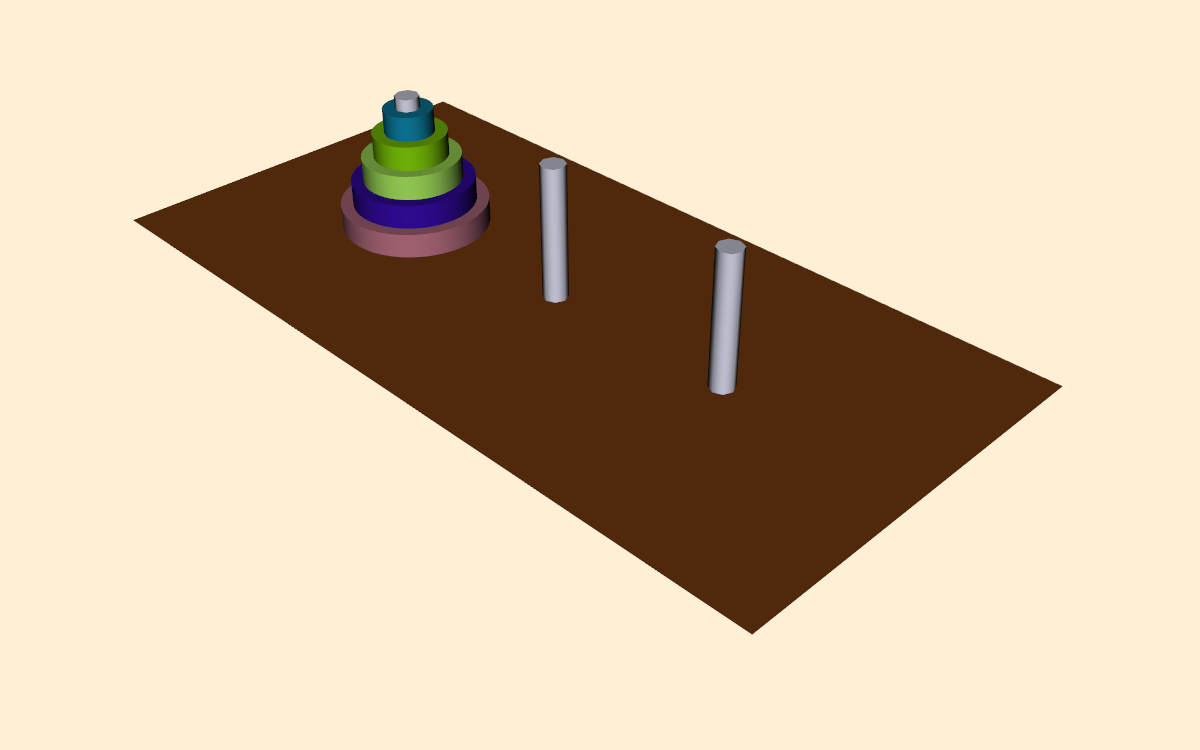
\includegraphics[width=\linewidth]{Figure12-20a}
		\caption{Initial (\href{https://lorensen.github.io/VTKExamples/site/Cxx/Visualization/HanoiInitial/}{HanoiInitial.cxx}) or (\href{https://lorensen.github.io/VTKExamples/site/Python/Visualization/HanoiInitial/}{HanoiInitial.py})}
		\label{fig:Figure12-20a}
	\end{subfigure}
	\hfill
	\begin{subfigure}[h]{0.54\linewidth}
		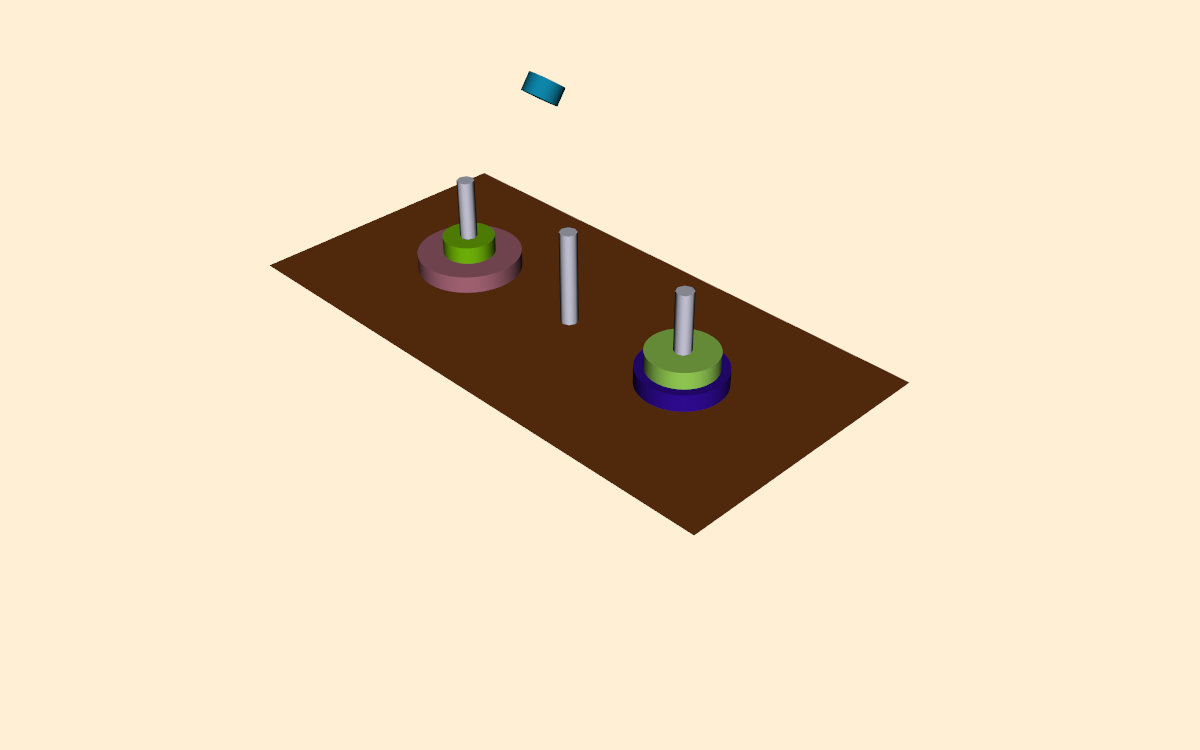
\includegraphics[width=\linewidth]{Figure12-20b}
		\captionsetup{justification=centering}
		\caption{Intermediate (\href{https://lorensen.github.io/VTKExamples/site/Cxx/Visualization/HanoiIntermediate/}{HanoiIntermediate.cxx}) or (\href{https://lorensen.github.io/VTKExamples/site/Python/Visualization/HanoiIntermediate/}{HanoiIntermediate.py})}
		\label{fig:Figure12-20b}
	\end{subfigure}
	\hfill
	\begin{subfigure}[h]{0.54\linewidth}
		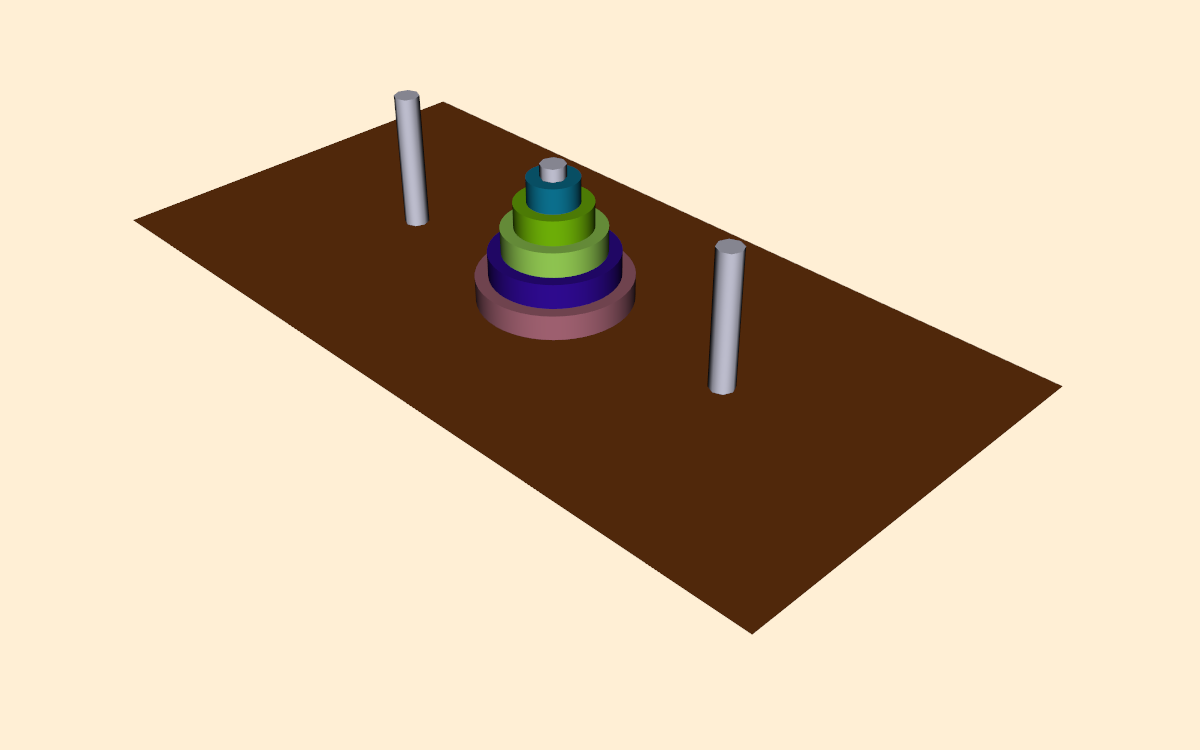
\includegraphics[width=\linewidth]{Figure12-20c}
        \captionsetup{justification=centering}
		\caption{Final (\href{https://lorensen.github.io/VTKExamples/site/Cxx/Visualization/Hanoi/}{Hanoi.cxx}) or (\href{https://lorensen.github.io/VTKExamples/site/Python/Visualization/Hanoi/}{Hanoi.py})}
		\label{fig:Figure12-20c}
	\end{subfigure}
    \captionsetup{justification=centering}
	\caption{Towers of Hanoi. (a) Initial configuration. (b) Intermediate configuration. (c) Final configuration.}\label{fig:Figure12-20}
\end{figure}

In this example we will visualize the operation of the recursive Towers of Hanoi\index{Towers of Hanoi|(} puzzle. In this puzzle there are three pegs (Figure \ref{fig:Figure12-20}). In the initial position there are one or more disks (or pucks) of varying diameter on the pegs. The disks are sorted according to disk diameter, so that the largest disk is on the bottom, followed by the next largest, and so on. The goal of the puzzle is to move the disks from one peg to another, moving the disks one at a time, and never placing a larger disk on top of a smaller disk.

The classical solution to this puzzle is based on a divide--and--conquer
approach \cite{AhoHopUll83}. The problem of moving \emph{$n$} disks from the
initial peg to the second peg can be thought of as solving two subproblems of size \emph{$n - 1$}. First move \emph{$n - 1$} disks from the initial peg to the third peg. Then move the $n$th disk to the second peg. Finally, move the \emph{$n - 1$} disks on the third peg back to the second
peg.

The solution to this problem can be elegantly implemented using recursion. We have shown portions of the C++ code below.
In the first part of the solution (which is not shown in the following ) the table top, pegs, and disks are created using the two classes vtkPlaneSource\index{vtkPlaneSource!application} and vtkCylinderSource\index{vtkCylinderSource!application}. The function Hanoi() is then called to begin the recursion.

\begin{lstlisting}[language=C++, caption={Recursive solution for the Towers of Hanoi.}]
// Recursive solution of Towers of Hanoi. Parameters are number
// of disks,originating peg, final peg, and intermediate peg.
staticvoidHanoi(intn,intpeg1,intpeg2,intpeg3)
{
  if(n!=1)
  {
  Hanoi(n-1,peg1,peg3,peg2);
  Hanoi(1,peg1,peg2,peg3);
  Hanoi(n-1,peg3,peg2,peg1);
  }
  else
  {
  MovePuck(peg1,peg2);
  }
}
\end{lstlisting}

The routine MovePuck() is responsible for moving a disk from one peg to another. It has been jazzed up to move the disk in small, user-specified increments, and to flip the disc over as it moves from one peg to the next. This gives a pleasing visual effect and adds the element of fun to the visualization.

\begin{lstlisting}[language=C++, caption={Moving the puck.}]
// Routine is responsible for moving disks from one peg to the next.
voidMovePuck(intpeg1,intpeg2)
{
  doubledistance, flipAngle;
  vtkActor*movingActor;
  int i;

  NumberOfMoves++;
  //get the actor t omove
  movingActor=(vtkActor*)pegStack[peg1].Pop();
  //get th edistance to move up
  distance=(H-(L*(pegStack[peg1].GetNumberOfItems()-1)) + rMax) /
    NumberOfSteps;
  for(i=0;i<NumberOfSteps;i++)
  {
  movingActor->AddPosition(0,distance,0);
  Renwin->Render();
  }

  //get the distance to move across
  distance=(peg2-peg1)*D/NumberOfSteps;
  flipAngle=180.0/NumberOfSteps;
  for(i=0;i<NumberOfSteps;i++)
  {
  movingActor->AddPosition(distance,0,0);
  movingActor->RotateX(flipAngle);
  Renwin->Render();
  }

  //get the distance to move down
  distance=((L*(pegStack[peg2].GetNumberOfItems()-1))-HrMax) /
    NumberOfSteps;
  for(i=0;i<NumberOfSteps;i++)
  {
  movingActor->AddPosition(0,distance,0);
  Renwin->Render();
  }
  pegStack[peg2].Push(movingActor);
}
\end{lstlisting}

Because of the clear relationship between algorithm and physical reality, the Towers of Hanoi\index{Towers of Hanoi|)} puzzle is relatively easy to visualize. A major challenge facing visualization researchers is to visualize more abstract information, such as information on the Internet, the structure of documents, or the effectiveness of advertising/entertainment in large market segments. This type of visualization, known as information visualization, is likely to emerge in the future as an important research challenge.
\index{algorithm visualization!application|)}\index{applications!algorithm visualization|)}
\index{applications|)}

\section{Chapter Summary}

This chapter presented several case studies covering a variety of visualization techniques. The examples used different data representations including polygonal data, volumes, structured grids, and unstructured grids. Both C++ and Tcl code was used to implement the case studies.

Medical imaging is a demanding application area due to the size of the input data. Three dimensional visualization of anatomy is generally regarded by radiologists as a communication tool for referring physicians and surgeons. Medical datasets are typically
image data --- volumes or layered stacks of 2D images that form volumes. Common visualization tools for medical imaging include isosurfaces, cut planes, and image display on volume slices.

Next, we presented an example that applied 3D visualization techniques to financial data. In this case study, we began by showing how to import data from an external source. We applied tube filters to the data and varied the width of the tube to show the volume of stock trading. We saw how different views can be used to present different pieces of information. In this case, we saw that by viewing the visualization from the front, we saw a conventional price display. Then, by viewing the visualization from above, we saw trade volume.

In the modelling case study we showed how to use polygonal models and the implicit modelling facilities in VTK to create a stylistic logo. The final model was created by extracting an isosurface at a user-selected offset.

Computational fluid dynamics analysts frequently employ structured grid data. We examined some strategies for exploring the scalar and vector fields. The computational grid created by the analyst serves as a starting point for analyzing the data. We displayed geometry extracted from the finite difference grid, scalar color mapping, and streamlines and streamtubes to investigate the data.

In the finite element case study, we looked at unstructured grids used in a simulation of a blow molding process. We displayed the deformation of the geometry using displacement plots, and represented the material thickness using color mapping. We saw how we can create simple animations by generating a sequence of images.

We concluded the case studies by visualizing the Towers of Hanoi algorithm. Here we showed how to combine the procedural power of C++ with the visualization capabilities in VTK. We saw how visualization often requires our creative resources to cast data structures and information into visual form.


\section{Bibliographic Notes}

The case studies presented in the chapter rely on having interesting data to visualize. Sometimes the hardest part of practicing visualizing is finding relevant data. The Internet is a tremendous resource for this task. Paul Gilste \cite{Gilster94} has written an excellent introduction to many of the tools for accessing information on the Internet. There are many more books available on this subject in the local bookstore.

In the stock case study we used a programming tool called AWK to convert our data into a form suitable for VTK. More information on AWK can be found in \emph{The AWK Programming Language} \cite{Aho88}. Another popular text processing languages is Perl \cite{Perl95}.

If you would like to know more about information visualization you can start with the references listed here \cite{Becker95} \cite{Ding90} \cite{Eick93} \cite{Feiner88} \cite{Johnson91} \cite{Robertson91}. This is a relatively new field but will certainly grow in the near future.

\printbibliography

\section{Exercises}
\label{exercises:ch_12}

\begin{enumerate}

	\item The medical example did nothing to transform the original data into a standard coordinate system. Many medical systems use RAS coordinates. R is right/left, A is anterior/posterior and S is Superior/Inferior. This is the patient coordinate system. Discuss and compare the following alternatives for transforming volume data into RAS coordinates. See (\href{https://lorensen.github.io/VTKExamples/site/Cxx/VisualizationAlgorithms/AnatomicalOrientation/}{AnatomicalOrientation.cxx}) and (\href{https://lorensen.github.io/VTKExamples/site/Python/VisualizationAlgorithms/AnatomicalOrientation/}{AnatomicalOrientation.py}).
	\begin{enumerate}
		\item vtkActor transformation methods.
		\item vtkTransformFilter.
		\item Reader transformations.
	\end{enumerate}

	\item Modify the last example found in the medical application (\href{https://lorensen.github.io/VTKExamples/site/Cxx/Medical/MedicalDemo3/}{MedicalDemo3.cxx}) or (\href{https://lorensen.github.io/VTKExamples/site/Python/Medical/MedicalDemo3/}{MedicalDemo3.py}) to use vtkImageDataGeometryFilter instead of
	vtkImageActor. Compare the performance of using geometry with using
	texture. How does the performance change as the resolution of the
	volume data changes?

	\item Modify the last medical example (\href{https://lorensen.github.io/VTKExamples/site/Cxx/Medical/MedicalDemo3/}{MedicalDemo3.cxx}) or (\href{https://lorensen.github.io/VTKExamples/site/Python/Medical/MedicalDemo3/}{MedicalDemo3.py}) to use vtkTexture and vtkPlaneSource instead of vtkImageActor.

	\item Change the medical case study to use dividing cubes for the skin surface.

	\item Combine the two scripts frogSegmentation.tcl and marchingFrog.tcl into one script that will handle either segmented or grayscale files. What other parameters and pipeline components might be useful in general for this application?

	\item Create polygonal / line stroked models of your initials and build your own logo. Experiment with different transformations.

	\item Enhance the appearance of Towers of Hanoi visualization.
	\begin{enumerate}
		\item Texture map the disks, base plane, and pegs.
		\item Create disks with central holes.
	\end{enumerate}

	\item Use the blow molding example as a starting point for the
	following.
	\begin{enumerate}
		\item Create an animation of the blow molding sequence. Is it possible to interpolate between time steps? How would you do this?
		\item Create the second half of the parison using symmetry. What   transformation matrix do you need to use?
	\end{enumerate}

	\item Start with the stock visualization example presented in this chapter.
	\begin{enumerate}
		\item Modify the example code to use a ribbon filter and linear extrusion filter as described in the text. Be careful of the width of the   generated ribbons.
		\item Can you think of a way to present high/low trade values for each day?
	\end{enumerate}

\end{enumerate}
